\documentclass[proquest]{uwthesis}[2014/11/13]
\usepackage{amsmath}
\usepackage{amsthm}
\usepackage{amssymb}
\usepackage[noadjust]{cite}
\usepackage{enumerate}
\usepackage{mathrsfs}
\usepackage{tikz}
\usepackage{tikz-cd}
\usepackage{wrapfig}
\usepackage{caption}
\usepackage[position=b]{subcaption}
\usepackage{hyperref}


\newtheorem{theorem}{Theorem}[section]
\newtheorem{prop}[theorem]{Proposition}
\newtheorem{lemma}[theorem]{Lemma}
\newtheorem{cor}[theorem]{Corollary}
\theoremstyle{definition}
\newtheorem{definition}[theorem]{Definition}
\newtheorem{question}[theorem]{Question}
\newtheorem{example}[theorem]{Example}
\newtheorem{defprop}[theorem]{Definition-Proposition}

\DeclareMathOperator{\Coh}{Coh}
\DeclareMathOperator{\Diag}{\underline{Diag}}
\DeclareMathOperator{\Ext}{Ext}
\DeclareMathOperator{\cExt}{\mathscr{E} \! \textit{xt}}
\DeclareMathOperator{\Gr}{Gr}
\DeclareMathOperator{\Hom}{Hom}
\DeclareMathOperator{\Ho}{H}
\newcommand{\cHom}{\mathcal{H} \textit{om}}
\DeclareMathOperator{\id}{id}
\DeclareMathOperator{\Ob}{Ob}
\DeclareMathOperator{\Sch}{{\bf Sch}}
\DeclareMathOperator{\Sh}{Sh}
\DeclareMathOperator{\Sing}{Sing}
\DeclareMathOperator{\Spec}{Spec}
\DeclareMathOperator{\Vect}{{\bf Vec}}
\DeclareMathOperator{\Zar}{Zar}

\renewcommand{\AA}{\mathcal{A}}
\newcommand{\BB}{\mathcal{B}}
\newcommand{\CC}{\mathbb{C}}
\newcommand{\CL}{\mathcal{C}}
\newcommand{\DD}{\mathcal{D}}
\newcommand{\EE}{\mathscr{E}}
\newcommand{\FF}{\mathscr{F}}
\newcommand{\GG}{\mathscr{G}}
\newcommand{\cH}{\mathscr{H}}
\newcommand{\HH}{\mathbb{H}}
\newcommand{\II}{\mathscr{I}}
\newcommand{\JJ}{\mathscr{J}}
\newcommand{\bL}{\textbf{L}}
\newcommand{\LL}{\mathcal{L}}
\newcommand{\MM}{\mathscr{M}}
\newcommand{\OO}{\mathcal{O}}
\newcommand{\PP}{\mathbb{P}}
\newcommand{\qis}{\simeq_{qis}}
\newcommand{\qisf}{\simeq_{qis,filt}}
\newcommand{\QQ}{\mathbb{Q}}
\newcommand{\RR}{\mathbb{R}}
\newcommand{\bR}{\textbf{R}}
\newcommand{\ZZ}{\mathbb{Z}}
\newcommand{\otimesL}{\otimes^{\bf L}}

\newcommand*\xbar[1]{%
  \hbox{%
    \vbox{%
      \hrule height 0.5pt % The actual bar
      \kern0.5ex%         % Distance between bar and symbol
      \hbox{%
        \kern-0.1em%      % Shortening on the left side
        \ensuremath{#1}%
        \kern-0.1em%      % Shortening on the right side
      }%
    }%
  }%
} 

\newcommand{\tu}{\underline{2}}
\DeclareMathOperator{\red}{red}
\newcommand{\DB}{\underline{\Omega}}
\newcommand{\db}{\underline{\omega}^\bullet}
\DeclareMathOperator{\tot}{tot}

\begin{document}
\prelimpages
\Title{Grothendieck Duality on Diagrams of Schemes}
\Author{Graham Clenaghan}
\Year{2015}
\Program{Mathematics}
\Chair{S\'andor Kov\'acs}{Professor}{Mathematics}
\Signature{Max Lieblich}
\Signature{James Zhang}

\copyrightpage
\titlepage

\abstract{%
	The Du Bois complex and Du Bois singularities, which extend results of Hodge theory to singular complex varieties, can be defined in terms of a cubical hyperresolution.
	In this dissertation I further develop the language of diagrams of schemes and then prove analogues of Grothendieck duality and other cohomological theorems for cubical diagrams.
	I then demonstrate the use of these by revisiting some known results about the Du Bois complex from a different perspective, and proving new results concerning the cohomology of a contraction.}
\tableofcontents

\textpages

\chapter{Introduction}
The Du Bois complex is a generalization of the de Rham complex of Hodge theory to singular complex varieties, and was introduced in \cite{Bois1981}.
The idea is to resolve the singularities of the variety and then push down the de Rham complex through this resolution, but a traditional resolution of singularities is inadequate for this process as topological information is lost.
Instead, hyperresolutions are an attempt to resolve the singularities of a variety while preserving the topology.

\begin{wrapfigure}{r}{0.15\textwidth}
	\centering
	\vspace{-20pt}
	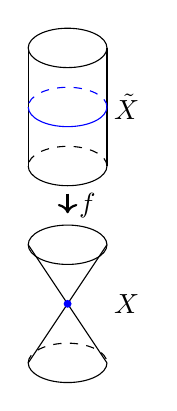
\begin{tikzpicture}[scale=0.5]
	\draw (-1,0) arc (180:360:1 and 0.5);
	\draw[dashed] (-1,0) arc (180:0:1 and 0.5);
	\draw (-1,0) -- (1, 3);
	\draw (1, 0) -- (-1, 3);
	\fill[blue] (0, 1.5) circle[radius=.1];
	\draw (1.5, 1.5) node {$X$};
	\draw (1, 3) arc (0:360: 1 and 0.5);
	
	\draw [thick,->] (0, 4.3) -- (0, 3.8);
	\draw (.5, 4) node {$f$};
	
	\draw (1,5) arc (360:180:1 and 0.5);
	\draw[dashed] (1,5) arc (0:180:1 and 0.5);
	\draw (1,5) -- (1,8);
	\draw (-1,5) -- (-1, 8);
	\draw[blue] (1, 6.5) arc (360:180: 1 and .5);
	\draw[dashed,blue] (1,6.5) arc (0:180:1 and .5);
	\draw (1.5, 6.5) node {$\tilde{X}$};
	\draw (1,8) arc (0:360: 1 and .5);
	\end{tikzpicture}
\end{wrapfigure}

As an example of this, consider the resolution of the cone over $\CC$, $f : \tilde{X} \rightarrow X$ obtained by blowing up the cone point, as seen in the figure on the right.
These topologically differ, as the cylinder has a non-trivial $\Ho^1 (\tilde{X}, \CC)$, while $\Ho^1 (X, \CC) = 0$, pishing the de Rham complex to $X$ naively would lose the property that $\Ho^i ( \tilde{X}, \CC) \cong \HH^i (\tilde{X}, \Omega_{\tilde{X}}^\bullet)$.

Instead, for a hyperresolution the goal is to ``remember" the fact that there is a $\PP^1$ in the cylinder which collapses to a point.
This is achieved by replacing the single scheme $\tilde{X}$ with a collection of schemes and maps between them which collectively make up the resolution.

Since the original definition, several implementations of the hyperresolution have been developed, each resulting in the same Du Bois complex. The most tractable definition is the cubical hyperresolution which uses diagrams of scheme, and such diagrams are the main topic of this dissertation.

Whichever way the complex is defined, Du Bois singularities are a natural condition of the 0-degree part of the complex $\DB_X^0$, which can be thought of as a hyperresolution version of rational singularities. In fact, Du Bois singularities generalize rational singularities as well as semi-log canonical singularities while maintaining features such as Kodaira vanishing.
If one prefers, there is a characterization due to Schwede \cite{Schwede2007} which allows Du Bois singularities to be defined without reference to hyperresolutions.

The main reference for diagrams of schemes is Guilli\'en, et. al \cite{Guillen1988}, and a restricted category of diagrams--only shape-preserving maps (defined in \ref{def:diagram}) are allowed--is studied in Hashimoto \cite{Lipman2009}.
Chapter \ref{chp:diagrams} serves as a mostly self-contained introduction to diagrams, and develops new tools we will use to tackle the main results.
Chapter \ref{chp:duboiscomplex} then introduces the Du Bois complex and singularities, and lists some known results.

The main results come in \ref{chp:grothendieckduality}, and consist of analogues of cohomological results from schemes including flat base change (theorem \ref{thm:flatbasechange}), the projection formula (theorem \ref{thm:projectionformula}), and Grothendieck duality (corollary \ref{cor:cubicalgrothdual}).
In particular, for the former there is an analogue of a dualizing complex on diagrams (herein called the canonical complex since it is not dualizing in the traditional sense), which when pushed to the resolved variety becomes the $\db_X$ Grothendieck dual of the complex $\DB_X^0$ which was studied somewhat in \cite{Kovacs2011a}.

Finally, in chapter \ref{chp:applications} there is some demonstration of these results outside the realm of diagrams of schemes, including the following theorem:
\begin{theorem}[Corollary \ref{cor:cohoofcontraction}]
	Let $X$ be a proper, reduced, Cohen-Macaulay $\CC$-scheme of dimension $n$ with Du Bois singularities, $Y$ smooth, with $f : Y \rightarrow X$ a proper morphism which is as isomorphism outside of a closed $p \in X$.
	Then, for $0 < i < n - 1$, the exceptional locus $Y_p$ satisfies
	\[
	H^i (Y_p, \DB_{Y_p}^0) = \begin{cases}
	\CC & \text{if } i = 0 \\
	0 & \text{if } 0 < i < n - 1.
	\end{cases}
	\]
	In particular, $Y_p$ is connected and if $Y_p$ has Du Bois singularities $H^i(Y_p, \OO_{Y_p}) = 0$ for $0 < i < n - 1$.
\end{theorem}



\chapter{Diagrams of Schemes and Their Sheaves}
\label{chp:diagrams}
\section{Diagram Categories and Diagrams of Schemes}
In general, a diagram in a given category $A$ will be a collection of objects in morphisms in that category; the idea is that we want to deal with that whole collection simultaneously. For example, in a cubical hyperresolution the diagram will contain both the resolution of singularities \textit{and} information about how the resolution map transforms the space.

These collections will be defined by a functor from another category $I$ to $A$, and in general any small $I$ and functor can work, but for our purposes we can restrict $I$ to a much simpler case:
\begin{definition}
	A \textit{diagram shape category} is a finite, thin (any two objects have at most one morphism between them) category without loops.
\end{definition}

It is clear why requiring finiteness makes things easier, the primary reason for requiring thinness is so that we can think of slice categories and over categories as fully faithful subcategories, which will make some constructions simpler.
Finally, loops in a thin category are somewhat silly (each map in the loop must be an isomorphism), so categories with loops contain no further information than the category with the loops collapsed, and doing so will be useful for lemma \ref{lem:affinecover}.
These conditions are particularly reasonable given the only categories we will be studying in much detail are given in definition \ref{def:cubicalcategories}.

\begin{definition}
	\label{def:diagram}
	Let $I$ be a diagram shape category and $A$ be any category.
	A \textit{diagram} in $A$ of shape $I$ (or an $I$-diagram) is a functor
	\[
		X_\bullet : I^{op} \rightarrow A.
	\]
	For each $\alpha$ and $\varphi$ an object and morphism from $I$ respectively, we'll write $X_\alpha$ and $X_\varphi$.
	
	A \textit{morphism} between an $I$-diagram $X_\bullet$ and a $J$-diagram $Y_\bullet$ is given by a \textit{shape functor} $\Gamma : I^{op} \rightarrow J^{op}$ and a natural transformation $\eta : X_\bullet \rightarrow Y_\bullet \circ \Gamma$.
	
	In simpler terms, this is a collection of morphisms between the components of $X_\bullet$ and $Y_\bullet$ such that the total diagram with all the arrows from the morphism and both diagrams drawn is commutative.
	Usually we'll denote a morphism as $f_\bullet : X_\bullet \rightarrow Y_\bullet$ with $\Gamma$ implicit and for each $\alpha \in I$, $f_\alpha : X_\alpha \rightarrow Y_{\Gamma(\alpha)}$.
	
	Call a morphism \textit{shape-preserving} if $\Gamma$ is the identity, and \textit{shape-embedding} if it is fully faithful.
	
	The category of diagrams in $A$ will be denoted $\Diag A$, and the category of $I$-diagrams with shape-preserving morphisms in $A$ will be denoted $\Diag_I A$.
	
	Finally, there is a diagonal functor for each $I$, $-\times I : A \rightarrow \Diag_I A$ sending each $X$ to the diagram $X \times I$ with shape $I$, all components $X$, and all morphisms the identity.
\end{definition}

The following definition introduces all the shapes we'll want to consider in detail.

\begin{definition}
	\label{def:cubicalcategories}
	Let $\underline{1}$ be the category $\{0\}$, and $\tu$ be the category $\{0 \rightarrow 1\}$.
	For $n \geq -1$, let $\Box_n^+$ be the product of $n+1$ copies of $\tu$.
	The elements here are tuples $\alpha = (\alpha_0, \dots, \alpha_n)$, with $\alpha_i \in \{0, 1\}$, and it is useful to define $|\alpha| = \sum \alpha_i$.
	Let $\Box_n$ be the full subcategory without the initial object $(0, \dots, 0)$.
	See figure \ref{fig:boxn}.
	
	A morphism of diagrams whose shape functor is the projection $\Box_n^{op} \times I^{op} \rightarrow I^{op}$ will be called a cubical morphism.
\end{definition}

\begin{figure}
	\centering
	\begin{subfigure}[t]{.2\textwidth}
		\centering
		\begin{tikzcd}[row sep=8, column sep=8]
			\circ
		\end{tikzcd}
	\end{subfigure}%
	\begin{subfigure}[t]{.25\textwidth}
		\centering
		\begin{tikzcd}[row sep=8, column sep=8]
			\bullet & & \arrow[dashed]{ll} \circ
		\end{tikzcd}
	\end{subfigure}%
	\begin{subfigure}[t]{.25\textwidth}
		\centering
		\begin{tikzcd}[row sep=8, column sep=8]
			\bullet & & \bullet \arrow{ll} \\ \\
			\bullet \arrow{uu} & & \circ \arrow[dashed]{ll} \arrow[dashed]{uu}
		\end{tikzcd}
	\end{subfigure}%
	\begin{subfigure}[t]{.3\textwidth}
		\centering
		\begin{tikzcd}[row sep=8, column sep=8]
			& \bullet \arrow[leftarrow]{dd}& & \arrow{ll} \bullet  \\
			\bullet \arrow{ur}& & \arrow[crossing over]{ll} \bullet \arrow{ur} \\
			& \bullet & & \arrow{ll} \bullet \arrow{uu}  \\
			\bullet \arrow{ur} \arrow{uu} & & \arrow[dashed]{ll} \circ \arrow[dashed]{ur} \arrow[dashed,crossing over]{uu}\\
		\end{tikzcd}
	\end{subfigure}
	\caption{For $n \in \{-1, 0, 1, 2\}$, $\Box_n^+$ is the diagram including the dashed arrows and an initial object, $\Box_n$ is the diagram without}
	\label{fig:boxn}
\end{figure}

With these generalities taken care of, we specialize to diagrams of schemes.

\begin{definition}
	A diagram of schemes is an object in the category $\Diag \Sch$.
	We'll say that a diagram of schemes $X_\bullet$ over $I$ (respectively, a morphism \mbox{$f_\bullet : X_\bullet \rightarrow Y_\bullet$}) has a given property $\mathcal{P}$ (e.g., smooth, noetherian) if for all $\alpha$, $X_\alpha$ (resp., $f_\alpha$) has $\mathcal{P}$.
\end{definition}
The following constructions will be needed later:

\begin{prop}
	\label{thm:fiberedprod}
	Let $f_\bullet : X_\bullet \rightarrow Y_\bullet$ and $g_\bullet : Y_\bullet\rq{} \rightarrow Y_\bullet$ be morphisms of diagrams of schemes.
	Then there is an inverse limit in the category of diagrams of schemes, the fibered product denoted $X_\bullet \times_{Y_\bullet} Y_\bullet\rq{}$ and fitting into the diagram
	\[
	\begin{tikzcd}
	X_\bullet \times_{Y_\bullet} Y_\bullet\rq{} \arrow{r}{f_\bullet\rq{}} \arrow{d}{g_\bullet\rq{}} & Y_\bullet\rq{} \arrow{d}{g_\bullet} \\
	X_\bullet \arrow{r}{f_\bullet} & Y_\bullet.
	\end{tikzcd}
	\]
	If each of the scheme maps in $f_\bullet$ has some property preserved under base change of schemes, then the scheme maps in $f_\bullet\rq{}$ have the same property.
\end{prop}
\begin{proof}
	First, we fix some notation: let $I$ be the shape of $X_\bullet$, $J$ the shape of $Y_\bullet\rq{}$, and $K$ the shape of $Y_\bullet$.
	Let $\Gamma : I \rightarrow K$ be associated to $f_\bullet$ and $\Lambda : J \rightarrow K$ be associated to $g_\bullet$.
	Then there is a fibered product $I \times_K J$ in the category of diagram shape categories: the full subcategory with objects $\{(i, j) \in I \times J : \Gamma(i) = \Lambda(j) \}$ in $I \times J$.
	
	Define an $I \times_K J$-scheme $X_\bullet\rq{}$ as follows: for $(i, j) \in I \times_K J$, let $X_{(i,j)}\rq{} = X_i \times_{Y_{\Gamma(i)}} Y_j$ and let the morphisms be the product of those in $X_\bullet$ and $Y_\bullet$.
	Then the collection of projections to each coordinate give the maps $f_\bullet\rq{}$ and $g_\bullet\rq{}$ in the diagram, and it is clear now $f_\bullet\rq{}$ preserves any property which is preserved under base change.
	
	Finally, we show this satisfies the universal property of the fibered product.
	If $Z_\bullet$ were an $L$-scheme with compatible morphisms to $X_\bullet$ and $Y_\bullet$, by definition it would have $\Theta_1 : L \rightarrow I$ and $\Theta_2 : L \rightarrow J$.
	For each $l \in L$, define a map $Z_l \rightarrow X_{(\Theta_1(l), \Theta_2(l))}\rq{}$ by the product of the morphisms to $X_{\Theta_1(l)}$ and $Y_{\Theta_2(l)}$.
\end{proof}

\begin{definition}
	\label{def:overscheme}
	Let $X_\bullet$ be an $I$-scheme.
	Suppose $\alpha \in I$ and $U \subseteq X_\alpha$.
	Define the {\it over-scheme of} $U$, $X_\bullet/U$ as a diagram of schemes over $\alpha/I$, the under category consisting of $(\beta, \phi)$ with $\beta \in I$ and $\phi : \alpha \rightarrow \beta$.
	The components are
	\[
	(X_\bullet/U)_{(\beta, \phi)} = X_\phi^{-1} (U) \subseteq X_\beta,
	\]
	and the maps are the restrictions of the maps of $X_\bullet$.
	There is a shape-embedding (by thinness) open immersion $i_U : X_\bullet / U \rightarrow X_\bullet$ mapping $X_\phi^{-1}(U) \hookrightarrow X_\beta$ for all $(\beta, \phi)$.
\end{definition}

\begin{definition}
	\label{def:diagrampreimage}
	Let $f_\bullet : X_\bullet \rightarrow Y_\bullet$ be a morphism of diagrams of schemes, with $U \subseteq Y_\alpha$.
	Define $f_\bullet^{-1}(U) = X_\bullet \times_{Y_\bullet} Y_\bullet / U$, and let $i_{f_\bullet^{-1} (U)}$ be the projection onto $X_\bullet$, which is a shape-embedding open immersion by thinness and proposition \ref{thm:fiberedprod}.
\end{definition}

\section{Sheaves on Diagrams}
With a definition of diagrams of schemes, we can now consider sheaves over diagrams, which can be thought of as compatible collections of sheaves and morphisms over the schemes in the diagram.

\begin{definition}[10.84 of \cite{Kollar2013}]
	Let $X_\bullet$ be an $I$-scheme.
	A sheaf $\FF_\bullet$ on $X_\bullet$ is a collection of sheaves $\FF_\alpha$ on $X_\alpha$ with, for each $\phi_{\alpha\beta} : X_\alpha \rightarrow X_\beta$ in the diagram, morphisms $\FF_\beta \rightarrow f_* \FF_\alpha$, or equivalently $f^* \FF_\beta \rightarrow \FF_\alpha$.
	This is an abelian category, so we can also take the derived category of such sheaves, $D(X_\bullet)$.
\end{definition}

Given a map of diagrams, there are several associated functors of sheaves, analogous to those on literal schemes.
The easiest to construct is the pullback

\begin{definition}
	Let $X_\bullet$ be an $I$-scheme and $Y_\bullet$ be a $J$-scheme, $f_\bullet : X_\bullet \rightarrow Y_\bullet$ be a morphism of diagrams of schemes over the functor $\Phi : I^{op} \rightarrow J^{op}$.
	Then if $\GG_\bullet$ is a sheaf over $Y_\bullet$, define the pullback $f^*_\bullet \GG_\bullet$ a sheaf on $X_\bullet$ as
	\[
	(f^*_\bullet \GG_\bullet)_\alpha = f_\alpha^* \GG_{\Phi(\alpha)}.
	\]
	This functor is right-exact and has a left-derived functor on the derived categories given on each component by
	\[
	(\bL f^*_\bullet G_\bullet)_\alpha = \bL f_\alpha^* G_{\Phi(\alpha)}.
	\]
\end{definition}

On the other hand, the pushforward is more mysterious, the problem being for each scheme in the target diagram, there are possibly many schemes mapping to it.
However, if this is the case then they form a diagram of sheaves over that target scheme, and we can define the pushforward as the limit of this diagram.

\begin{definition}
	\label{def:pushforward}
	Let $X_\bullet$ be an $I$-scheme and $Y_\bullet$ a $J$-scheme, $f_\bullet : X_\bullet \rightarrow Y_\bullet$ a morphism of diagrams of schemes over the functor $\Phi : I^{op} \rightarrow J^{op}$.
	Then if $\FF_\bullet$ is a sheaf over $X_\bullet$, define the pushforward $f_{\bullet*} \FF_\bullet$ a sheaf on $Y_\bullet$ as
	\[
	(f_{\bullet*} \FF_\bullet)_\alpha = \varprojlim_{(\beta, \phi)} Y_{\phi *} f_{\beta *} \FF_\beta,
	\]
	where $(\beta, \phi)$ ranges over $\beta \in I$ and $\phi : \Phi(\beta) \rightarrow \alpha$ a morphism in $J$.
	This functor is left-exact and has a right-derived functor on the derived categories given on each component by
	\[
	(\bR f_{\bullet*} F_\bullet)_\alpha = \bR \varprojlim_{(\beta, \phi)} \bR Y_{\phi *} \bR f_{\beta *} F_\beta.
	\]
\end{definition}

\begin{prop}[I 5.5 of \cite{Guillen1988}]
	With these definitions and using this notation, $f_{\bullet *}$ is the right adjoint of $f_\bullet^*$ and $\bR f_{\bullet *}$ is the right adjoint of $\bL f_\bullet^*$.
\end{prop}



The main case of interest is a hyperresolution of a literal scheme, so it is worth considering in the case where $J = \underline{1}$, and even more particular where $I = \Box_n$.
After this first restriction, the functor $\bR f_{\bullet *}$ can be written as
\[
\bR f_{\bullet*} F_\bullet = \bR \varprojlim_\beta \bR f_{\beta *} F_\beta
\]

Restricting to $I = \Box_n$ is very powerful, as we will see in section \ref{sec:cubicaldescent}.

The following gives a notion of global sections for sheaves on diagrams:

\begin{definition}
	If $X_\bullet$ is a diagram of schemes, $\FF_\bullet$ a sheaf on $X_\bullet$, then define the functor
	\[
	\Gamma(X_\bullet, \FF_\bullet) = \varprojlim \Gamma(X_\alpha, \FF_\alpha).
	\]
	Similarly, if $F_\bullet \in D(X_\bullet)$, define
	\[
	\bR \Gamma(F_\bullet) = \bR \varprojlim \bR \Gamma(F_\alpha).
	\]
	Note that if $f_\bullet : X_\bullet \rightarrow \Spec k$ is a morphism to a field, $\Gamma = f_{\bullet *}$.
\end{definition}

Given $\FF_\bullet$ and $\GG_\bullet$, sheaves on $X_\bullet$, we can define $\Hom_{X_\bullet}(\FF_\bullet, \GG_\bullet)$ as the morphisms in the category of sheaves, and this has many of the properties as before, however defining a sheaf $\cHom_{X_\bullet}(\FF_\bullet, \GG_\bullet)$ is more subtle as the most obvious choice does not have the natural maps required.
\begin{definition}
	Let $X_\bullet$ be a diagram of schemes, $\FF_\bullet$ and $\GG_\bullet$ two sheaves over $X_\bullet$.
	Define $\cHom_{X_\bullet}(\FF_\bullet, \GG_\bullet)$ as follows: for each $\alpha \in I$, and $U \subseteq X_\alpha$ open, let
	\[
	(\cHom_{X_\bullet}(\FF_\bullet, \GG_\bullet))_\alpha(U) = \Hom_{X_\bullet/U} ( i_U^* \FF_\bullet , i_U^* \GG_\bullet).
	\]
	Note that $X_\bullet/U$ and $i_U$ are defined in \ref{def:overscheme}. This gives a sheaf on each $X_\alpha$.
	For $X_\phi : X_\alpha \rightarrow X_\beta$, $U \subseteq X_\beta$, there is a map $X_\bullet / \phi^{-1}(U) \rightarrow X_\bullet / U$ such that the $i$ maps commute, and putting this together gives maps $(\cHom_{X_\bullet}(\FF_\bullet, \GG_\bullet))_\beta(U) \rightarrow (\cHom_{X_\bullet}(\FF_\bullet, \GG_\bullet))_\alpha(X_\phi^{-1}(U))$ as needed.
\end{definition}

\begin{prop}
	Let $X_\bullet$ be a diagram of schemes, $\FF_\bullet$ and $\GG_\bullet$ two sheaves over $X_\bullet$.
	Then
	\[
	\Gamma(X_\bullet, \cHom_{X_\bullet}(\FF_\bullet, \GG_\bullet)) = \Hom_{X_\bullet}(\FF_\bullet, \GG_\bullet),
	\]
	and similarly if $F_\bullet, G_\bullet \in D^+(X_\bullet)$
	\[
	\bR \Gamma (\bR \cHom_{X_\bullet}(F_\bullet, G_\bullet)) = \bR \Hom_{X_\bullet}(F_\bullet, G_\bullet).
	\]
\end{prop}
\begin{proof}
	Note that $ \Hom_{X_\bullet / X_\alpha} ( i_{X_\alpha}^* \FF_\bullet , i_{X_\alpha}^* \GG_\bullet)$ consists of compatible morphisms of sheaves $\FF_\beta \rightarrow\nobreak \GG_\beta$ for each $\beta$ under $\alpha$, but then it is clear the inverse limit of these groups will be the collection of compatible morphisms $\FF_\beta \rightarrow \GG_\beta$ for all $\beta$, which is precisely $\Hom_{X_\bullet}(\FF_\bullet, \GG_\bullet)$.
	
	The derived category version is simply by the composition of derived functors.
\end{proof}

The following proposition can be thought of as a generalization of the above, where $\Gamma$ is thought of as a special case of the pushforward functor. 
The natural map obtained by this characterization is used in the sheaf version of duality.

\begin{prop}
	\label{thm:chomnatmap}
	Let $f_\bullet : X_\bullet \rightarrow Y_\bullet$ be a morphism of diagrams of schemes, and $\FF_\bullet$, $\GG_\bullet$ two $X_\bullet$ sheaves.
	Then there is a natural isomorphism, for each $U \subseteq Y_\alpha$
	\[
	f_{\bullet *}  \cHom_{X_\bullet} (\FF_\bullet, \GG_\bullet) (U) \xrightarrow{\sim} \Hom_{f_\bullet^{-1}(U)} ( i_{f_\bullet^{-1}(U)}^* \FF_\bullet, i_{f_\bullet^{-1}(U)}^* \GG_\bullet).
	\]
	
	Furthermore, there is a natural map
	\[
	f_{\bullet *} \cHom_{X_\bullet} (\FF_\bullet , \GG_\bullet) \rightarrow \cHom_{Y_\bullet} (f_{\bullet *} \FF_\bullet, f_{\bullet *} \GG_\bullet),
	\]
	and its derived version
	\[
	\bR f_{\bullet *} \bR \cHom_{X_\bullet} (F_\bullet , G_\bullet) \rightarrow \bR \cHom_{Y_\bullet} (\bR f_{\bullet *} F_\bullet, \bR f_{\bullet *} G_\bullet).
	\]
\end{prop}
\begin{proof}
	Working through the definitions,
	\[
	f_{\bullet *}  \cHom_{X_\bullet} (\FF_\bullet, \GG_\bullet) (U) = \varprojlim_{(\beta, \phi)} \Hom_{X_\bullet / f_\beta^{-1}(Y_\phi^{-1}(U)} (i_{f_\beta^{-1}(Y_\phi^{-1}(U)}^* \FF_\bullet, i_{f_\beta^{-1}(Y_\phi^{-1}(U)}^* \GG_\bullet).
	\]
	The elements on the left are tuples of compatible morphisms of sheaves $(\psi_{(\beta, \phi)})$, where $(\beta, \phi)$ ranges over $I \times_J \alpha/J$.
	$f_\bullet^{-1}(U)$ is a $I \times_J \alpha/J$ scheme, and working through the definitions, $(p_{f_\bullet^{-1}(U)}^* \FF_\bullet)_{(\beta, \phi)} = \FF_\beta |_{f^{-1}_\beta(Y_\phi^{-1}(U))}$, then $\psi_{(\beta, \phi)}$ gives a morphism from this to $(p_{f_\bullet^{-1}(U)}^* \GG_\bullet)_{(\beta, \phi)}$ for each $(\beta, \phi)$, and these maps are compatible.
	
	The inverse is the restriction of the morphism $i_{f_\bullet^{-1}(U)}^* \FF_\bullet \rightarrow i_{f_\bullet^{-1}(U)}^* \GG_\bullet$ to each of the components of the limit.
	
	To define the natural map, we can define compatible maps of the $U$ sections, and by the first part and the definition, these are maps
	\[
	\Hom_{f_\bullet^{-1}(U)} ( i_{f_\bullet^{-1}(U)}^* \FF_\bullet, i_{f_\bullet^{-1}(U)}^* \GG_\bullet) \rightarrow \Hom_{Y_\bullet / U} (i_U^* f_{\bullet *} \FF_\bullet, i_U^* f_{\bullet *} \GG_\bullet).
	\] 
	On each of the components, $i_U^*$ and $i_{f_\bullet^{-1}(U)}^*$ are just the restrictions, which $f_{\bullet *}$ is compatible with, so we can rewrite the right side as
	\[
	Hom_{Y_\bullet / U} (f_{\bullet *} i_{f_\bullet^{-1}(U)}^*\FF_\bullet,  f_{\bullet *} i_{f_\bullet^{-1}(U)}^*\GG_\bullet).
	\]
	Then it is clear the natural map is just the application of the functor $f_{\bullet *}$.
	
	The derived version is then tediously obtained by the sheaf version.
\end{proof}


\begin{prop}
	Let $X_\bullet$ be a diagram of schemes, $i_\bullet : U_\bullet \hookrightarrow X_\bullet$ a flat shape-embedding.
	Then $i_\bullet^*$ is an exact functor.
\end{prop}
\begin{proof}
	Let the shape functor of $i_\bullet$ be the inclusion of $J \hookrightarrow I$.
	Treat $i_\bullet$ as a composition of a flat, shape-preserving map $U_\bullet \rightarrow X_\bullet|_J$ and the inclusion $X_\bullet|_J \rightarrow X_\bullet$.
	By \cite{Lipman2009}, II 6, the restriction functor to any subdiagram is exact (indeed, it has both left and right adjoints), and the pullback by a shape-preserving map is just the pullback on each component, and on each component it is exact.
\end{proof}

It's tempting to think of complexes in the derived category of sheaves on a diagram as a sort of diagram of complexes in the derived categories of sheaves on the component schemes: an object $F_\alpha \in D(X_\alpha)$ and compatible morphisms $\bR X_{\phi_{\beta \alpha} *} F_\beta \rightarrow F_\alpha$.
This is a subtle issue: the complex category $C(\Sh(X_\bullet))$ is indeed this sort of construction, but the chain homotopies over the entire diagram are not the same as the chain homotopies over each component combined, they must be compatible as well.
Here is a simple example of this phenomenon:
\begin{example}
	\label{ex:ddiagvsdiagd}
	Consider the diagram of schemes $X_\bullet = (\Spec k \rightarrow \Spec k)$ over the category $\tu$, and the following elements, of the complex category, $F_\bullet$:
	\[
		\begin{tikzcd}[column sep = small, row sep = small]
			\cdots \ar[r] & 0 \ar[r] \ar[d] & 0 \ar[r] \ar[d] & k \ar{r} \ar{d} & k \ar[r] \ar[d] & 0 \ar[r] \ar[d] & \cdots \\
			\cdots \ar[r] & 0 \ar[r] & 0 \ar[r] & k \ar[r] & 0 \ar[r] & 0 \ar[r] & \cdots,
		\end{tikzcd}
	\]
	and $G_\bullet$:
	\[
		\begin{tikzcd}[column sep = small, row sep = small]
			\cdots \ar[r] & 0 \ar[r] \ar[d] & 0 \ar[r] \ar[d] & k \ar[r] \ar[d] & 0 \ar[r] \ar[d] & 0 \ar[r] \ar[d] & \cdots \\
			\cdots \ar[r] & 0 \ar[r] & k \ar[r] & k \ar[r] & 0 \ar[r] & 0 \ar[r] & \cdots.
		\end{tikzcd}
	\]
	The chain maps between $F_\bullet$ and $G_\bullet$ are exactly what we think, chain maps between the two top rows and chain maps between the two bottom that are compatible, and thus $\Hom_{C(X_\bullet)}(F_\bullet, G_\bullet) = k$.
	Next, to compute the $\Hom$ in the derived category, since everything is injective here, we need only mod out by chain homotopy.
	When we ignore the compatibilities, and just consider each of $F_\bullet$ and $G_\bullet$ as two elements of $D(\Spec k)$ and a morphism between them, then we can replace the top row of $F_\bullet$ and the bottom row of $G_\bullet$ with 0 as these rows are quasi-isomorphic to 0, thus the $\Hom$ considered this way would itself be zero.
	However, the only nontrivial maps of the homotopy must fit into diagrams like
	\[
		\begin{tikzcd}
			k \arrow{r}{h} \ar[d] & k \ar[d] \\
			0 \ar[r] & k,
		\end{tikzcd}
	\]
	and therefore must be zero, so in fact $\Hom_{D(X_\bullet)}(F_\bullet, G_\bullet) = k$.
	
	Another thing to note about this is that $F_\bullet$ is not quasi-isomorphic to the complex 
	\[
	\begin{tikzcd}[column sep = small, row sep = small]
	\cdots \ar[r] &  0 \ar[r] \ar[d] & 0 \ar{r} \ar{d} & 0 \ar[r] \ar[d] & \cdots \\
	\cdots \ar[r] & 0 \ar[r] & k \ar[r] & 0 \ar[r] & \cdots,
	\end{tikzcd}
	\]
	as any morphism to or from this complex runs into the same issue: some subdiagram commuting meaning the map must be zero.
\end{example}
	
\section{Cubical Descent}
\label{sec:cubicaldescent}

As previously mentioned, we are particularly interested in the case of a $\Box_n$-diagram.
This has particularly nice properties in that the $\bR \varprojlim$ functor which is relatively mysterious in general becomes very concrete and even computable, it is given by the so-called simple functor, which appears in \cite{Guillen1988} I 6 and is developed further in \cite{Guillen2002} (an English reference is given by \cite{Pascual2009}).

For notational convenience, we'll consider $\Box_n = \{(\alpha_0, \dots \alpha_n) : \alpha_i \in \{0, 1\}\})$ as a subset of $\ZZ^n$.
Let $e_i$ be the $i$th basis vector of $\ZZ^n$, and let the morphism from $\alpha$ to $\alpha + e_i$ (which exists if and only if $\alpha_i = 0$ be denoted by $\phi_{(\alpha, i)}$.

\begin{definition}[\cite{Guillen1988} I 6]
	Let $F_\bullet : \Box_n \rightarrow C(A)$ be a diagram (over $\Box_n^{op}$) in the category of complexes in an abelian category $A$, where the differential of $F_\alpha$ is $d_\alpha$.
	Define the {\it simple complex} of $s(F_\bullet)$ to be the object in $C(A)$ with
	\[
	s(F_\bullet)^p = \bigoplus_\alpha F_\alpha^{p+1-|\alpha|}
	\] 
	and such that the differential on each $F_\alpha^{p+1-|\alpha|}$ is
	\[
	d = (\bigoplus_{\{i : \alpha_i = 0\}} (-1)^{\sum_{j < i} \alpha_j} F_{\phi_{(\alpha, i)}}) \oplus (-1)^{|\alpha|} d_\alpha.
	\]
\end{definition}

In more tangible terms, complex is obtained by combining all the complexes, staggering them to the right by the value of $|\alpha|$.
To illustrate, suppose $\Phi$ was the $\Box_1$-diagram
\[
\begin{tikzcd}
C^\bullet & \arrow{l} A^\bullet \\
B^\bullet \arrow{u}.
\end{tikzcd}
\]
Then to obtain the simple complex, we arrange the complexes, written out, as
\[
\begin{tikzcd}
\cdots \arrow{r}{-} &  A^0 \arrow{r}{-} \arrow{dr}{+} & A^1 \arrow{r}{-} \arrow{dr}{+} & A^2 \arrow{r}{-} \arrow{dr}{+} & \cdots \\
& \cdots \arrow{r}{+} & C^0 \arrow{r}{+} & C^1 \arrow{r}{+} & C^2 \arrow{r}{+} & \cdots \\
\cdots \arrow{r}{-} & B^0 \arrow{r}{-} \arrow{ur}{-} & B^1 \arrow{r}{-} \arrow{ur}{-} & B^2 \arrow{r}{-} \arrow{ur}{-} & \cdots
\end{tikzcd}
\]
and then take the direct sum of each column, with the signs above indicating the sign in the differential.

This can also be interpreted as taking a succession of mapping cones: treat $F_\bullet$ as a $(\Box_n^+)^{op}$-diagram with a 0 at the initial object, then since by definition $\Box_n^+ = \prod \tu$, $s$ on $\tu$ is the mapping cone, and by either direct computation or as in \cite{Guillen2002} $s$ factors over products.

\begin{prop}[\cite{Guillen1988} I 6.3, \cite{Guillen2002} 1.3.1]
	Let $A$ be an abelian category, then the simple complex is a functor $s:\Diag_{\Box_n} C(A) \rightarrow C(A)$ which takes quasi-isomorphisms to quasi-isomorphisms.
	
	Then this functor descends to the derived categories $D(\Diag_{\Box_n} A)$ and $\Diag_{\Box_n} D(A)$ and is the same when considering an object of the first as an object of the latter (so that the issues arising in example \ref{ex:ddiagvsdiagd} vanish when this functor is applied).
\end{prop}
\begin{prop}
	\label{thm:simple}
	Let $X_\bullet$ be a $\Box_n$-scheme with a map $f_\bullet : X_\bullet \rightarrow X$ to a scheme, and let $F_\bullet$ be an element of the bounded below derived category of sheaves on $\Box_n$
	Then $\bR f_{\bullet *} F_\bullet$ is naturally quasi-isomorphic to the simple complex formed by the $\Box_n$ diagram of $\bR f_{\alpha *} F_\alpha$ for each $\alpha \in \Box_n$.
\end{prop}
\begin{proof}
	This is I 6.6 of \cite{Guillen1988} in the special case of $I = \underline{1}$, and $K_\bullet$ the functor sending 0 to $\Box_n$.
\end{proof}

This works just as well for functors $\Box_n \rightarrow C(A)$ (i.e. objects of $\Diag_{\Box_n^{op}} C(A)$).
To avoid confusion, we notate this differently:
\begin{definition}
	Let $F_\bullet \in \Diag_{\Box_n} C(A)$, define the complex $s^*(F_\bullet)$ via
	\[
		s^*(F_\bullet)^p = \oplus_\alpha F_\alpha^{p-1+|\alpha|}
	\]
	with differential on each $F_\alpha^{p-1+|\alpha|}$
	\[
		d = \bigoplus_{(i : \alpha_i = 0)} (-1)^{\sum_{j < i} \alpha_j} F_{\phi(\alpha,i)} \oplus (-1)^{|\alpha|} d_\alpha.
	\]
	
	Proposition \ref{thm:simple} holds for $s^*$ as well.
\end{definition}

The functors $s$ and $s^*$ have a sort of duality theorem:

\begin{theorem}
	\label{thm:simpleduality}
	Let $A$ be an abelian category, $F_\bullet \in D(\Diag_{\Box_n^{op}} A)$ and $G \in D(A)$, then $\bR \Hom(F_\bullet, G \times \Box_n^{op})$ is a $\Box_n$-diagram, $\bR \Hom(G \times \Box_n, F_\bullet)$ is a $\Box_n^{op}$-diagram and
	\begin{align*}
		\bR \Hom(s(F_\bullet), G) &= s^* (\bR \Hom(F_\bullet, G \times \Box_n^{op})) \\
		\bR \Hom(G, s(F_\bullet)) &= s (\bR \Hom(G \times \Box_n^{op}, F_\bullet))
	\end{align*}
	
	If $F \in D(A)$, $G_\bullet \in D(\Diag_{\Box_n} A)$, then the analogous equalities hold:
	
	\begin{align*}
		\bR \Hom(F, s^* (G_\bullet)) &= s^* (\bR \Hom(F \times \Box_n, G_\bullet)) \\
		\bR \Hom(s^*(G_\bullet), F) &= s(\bR \Hom(G_\bullet, F \times \Box_n))
	\end{align*}
	
	Furthermore, this continues to hold if $A$ is a category of sheaves and we use sheaf $\cHom$.
\end{theorem}
\begin{proof}
	These are all similar proofs, both in technique and tediousness, so we check the first only.
	
	Choose representatives of $F_\bullet$ and $G$ in $K(\Diag_{\Box_n^{op}} A)$ and $K(A)$ respectively, with $G$ K-injective.
	Then $\bR \Hom(F, s^* (G_\bullet)$ is represented by the complex with degree $p$ given by
	\begin{align*}
		\bR \Hom(F, s^* (G_\bullet))^p &= \bigoplus_{i-j = p} \Hom(s(F_\bullet)^j, G^i) \\
		&= \bigoplus_{i-j = p} \Hom(\bigoplus_\alpha F_\alpha^{j + 1 - |\alpha|}, G^i) \\
		&= \bigoplus_\alpha \bigoplus_{i-j = p} \Hom(F_\alpha^{j + 1 - |\alpha|}, G^i) \\
		&= \bigoplus_\alpha \bigoplus_{i-k = p - 1 + |\alpha|} \Hom(F_\alpha^k, G^i) \\
		&= \bigoplus_\alpha \bR \Hom(F_\alpha, G)^{p-1+|\alpha|} \\
		&= s^* (\bR \Hom(F_\bullet, G \times \Box_n^{op}))^p.
	\end{align*}
	Furthermore, the differentials of the two complexes also agree after enough identifications.
\end{proof}

We can skip the simple complex in actual computations by using the following spectral sequence.

\begin{prop}[\cite{Guillen1988} I 6.7]
	\label{prp:cubicalcohospecseq}
	Let $X_\bullet$ be a $\Box_n$-scheme, and $F_\bullet \in D(X_\bullet)$.
	Then there is a spectral sequence computing the cohomology of $F_\bullet$:
	\[
	E_1^{pq} = \bigoplus_{|\alpha| = p + 1} \HH^q(X_\alpha, F_\alpha) \Rightarrow \HH^{p+q}(X_\bullet, F_\bullet).
	\]
	For a morphism $\pi_\bullet : X_\bullet \rightarrow X$ to a scheme $X$, this generalizes to a spectral sequence
	\[
	E_1^{pq} = \bigoplus_{|\alpha| = p + 1} \bR^q \pi_{\alpha *}F_\alpha \Rightarrow \bR^{p+q} \pi_{\bullet *} F_\bullet.
	\]
\end{prop}

\section{Cubical Hyperresolutions}

The basic unit of a cubical hyperresolution is a 2-resolution: this can be thought of a resolution of singularities which keeps track of the fiber over the singular locus.

\begin{definition}[10.76 of \cite{Kollar2013}]
	If $X$ is an $I$-scheme, then a {\it 2-resolution} of $S$ is a $\Box_1^+ \times I$-scheme $X_\bullet$ as in the diagram
	\[
	\begin{tikzcd}
	X_{11} \arrow[hook]{r} \arrow{d} & X_{01} \arrow{d}{f} \\
	X_{10} \arrow[hook]{r} & X_{00}
	\end{tikzcd}
	\]
	such that the horizontal maps are closed immersions, $f$ is a resolution of singularities which is an isomorphism outside of $X_{10} \subseteq X_{00}$, and $X_{11}$ is the fibered product.
\end{definition}

Any resolution of $X$ can be completed to a 2-resolution by adding the singular set and its pullback.
For instance, we can improve the resolution of the cone by forming the square as pictured on the right.

\begin{wrapfigure}{r}{.25\textwidth}
	\centering
	\vspace{-25pt}
	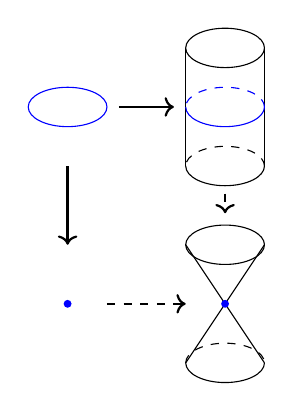
\begin{tikzpicture}[scale=0.5]
	\draw[blue](-3, 6.5) arc (0:360: 1 and .5);
	
	\draw [thick, ->] (-2.7, 6.5) -- (-1.3, 6.5);
	
	\draw [thick,->] (-4, 5) -- (-4, 3);
	
	\fill[blue] (-4, 1.5) circle[radius=.1];
	
	\draw [thick, dashed, ->] (-3, 1.5) -- (-1, 1.5);
	
	\draw (-1,0) arc (180:360:1 and 0.5);
	\draw[dashed] (-1,0) arc (180:0:1 and 0.5);
	\draw (-1,0) -- (1, 3);
	\draw (1, 0) -- (-1, 3);
	\fill[blue] (0, 1.5) circle[radius=.1];
	\draw (1, 3) arc (0:360: 1 and 0.5);
	
	\draw [thick,dashed,->] (0, 4.3) -- (0, 3.8);
	
	\draw (1,5) arc (360:180:1 and 0.5);
	\draw[dashed] (1,5) arc (0:180:1 and 0.5);
	\draw (1,5) -- (1,8);
	\draw (-1,5) -- (-1, 8);
	\draw[blue] (1, 6.5) arc (360:180: 1 and .5);
	\draw[dashed,blue] (1,6.5) arc (0:180:1 and .5);
	\draw (1,8) arc (0:360: 1 and .5);
	\end{tikzpicture}
	\vspace{-15pt}
\end{wrapfigure}

Now if we consider the $\Box_1$-shaped diagram without the cone and dashed maps, all the varieties are smooth and yet the necessary information about the singularity is preserved, in fact the cone is now the pushout of this diagram.

In this example, and for any variety $X$ where $\Sing X$ and it's pullback is smooth, the first 2-resolution will be enough, but in general the process will need to continue to resolve the singularities of $\Sing X$.
Since we would like the final product to be a diagram, we first define a way to combine successive 2-resolutions into a larger diagram

\begin{definition}[10.78 of \cite{Kollar2013}]
	Suppose $n \leq 1$, $X^r_\bullet$ a $\Box^+_r \times I$-scheme for $1 \leq r \leq n$ such that $X_{00\bullet}^{r+1}$ is equal to $X_{1\bullet}^r$.
	That is, each term in the sequence is a 2-resolution of the left part of the previous diagram.
	Then define the {\it reduction}, a $\Box_n^+ \times I$-scheme $\red(X_\bullet^1, \dots, X_\bullet^n)$ inductively as follows:
	\begin{align*}
		\red(X_\bullet^1, X_\bullet^2) &= 
		\begin{cases}
			X^1_{0\beta} & \alpha = (0,0) \\
			X^2_{\alpha\beta} & \alpha \in \Box_1
		\end{cases} \\
		\red(X_\bullet^1, \dots, X_\bullet^n) &= \red(\red(X_\bullet^1, \dots, X_\bullet^{n-1}), X^n_\bullet).
	\end{align*}
\end{definition}

Now we come to the definition of a hyperresolution:

\begin{definition}[10.79 of \cite{Kollar2013}]
	Let $X$ be an $I$-scheme.
	Then the $\Box_n^+ \times I$-scheme $\red(X_\bullet^1, \dots, X_\bullet^n)$ is a {\it cubic hyperresolution of $X$} if $X_\bullet^1$ is a 2-resolution of $X$, each successive step is a 2-resolution of the left part of the last, and each scheme in the final diagram is smooth.
	Often, this will be written as a map $f_\bullet : X_\bullet \rightarrow X$, where $X_\bullet$ is a $\Box_n \times I$-scheme, and the total diagram of $X_\bullet \rightarrow X$ is the cubic hyperresolution.
\end{definition}

\begin{theorem}[I 2.15 of \cite{Guillen1988}]
	\label{thm:hyperexist}
	Suppose $I$ is a finite, ordered category, and $X$ is an $I$-scheme over a field of characteristic 0.
	Then there exists a cubic hyperresolution $X_\bullet$ of $X$ such that for each $\alpha \in \Box_n$
	\[
	\dim X_\alpha \leq \dim X - |\alpha| + 1.
	\]
\end{theorem}

\begin{prop}
	Suppose $\pi_\bullet : Y_\bullet \rightarrow X_\bullet$ is a cubical hyperresolution of the $I$-scheme $X_\bullet$, and $\xbar{X}_\bullet \rightarrow X_\bullet$ is a shape-embedding morphism of diagrams, an isomorphism on each component of $\xbar{X}_\bullet$.
	Then $Y_\bullet \times_{X_\bullet} \xbar{X}_\bullet \rightarrow \xbar{X}_\bullet$ is a cubical hyperresolution of $\xbar{X}_\bullet$.
\end{prop}
\begin{proof}
	Take the sequence of 2-resolutions which gives $\pi_\bullet$ as cubical hyperresolutions, then the fibered product of each of these remains a 2-resolution as closed immersions, birational maps, and fibered products are all preserved.
	Finally, the reduction of this sequence gives $Y_\bullet \times_{X_\bullet} \xbar{X}_\bullet$.
\end{proof}
	
\section{Grothendieck Topology}
Everything done so far can be recovered by viewing diagrams of schemes as a certain type of site and using the definition of sheaves on a site.
For instance, the sheaf-hom defined above is exactly the sheaf-hom over a site.
\begin{defprop}
	For any diagram of schemes $X_\bullet$, define the Zariski site $\Zar(X_\bullet)$ to be the category of shape-embedding open immersions $U_\bullet \rightarrow X_\bullet$, with morphisms compatible shape-embedding open immersions $U_\bullet \rightarrow V_\bullet$.
	
	For each $U_\bullet$, a set of maps $\{U_{\bullet i} \rightarrow U_\bullet\}$ in the category is a covering if each component of $U_\bullet$, $U_\alpha$ is covered by the set of components $\{U_{\alpha i}\}$.
	These form a Grothendieck topology, and a morphism of the diagrams gives an associated morphism of the Zariski sites, and the category of sheaves over $X_\bullet$ is equivalent to the category of sheaves on $\Zar(X_\bullet)$, and each morphism of diagrams has an associated morphism of sites.
\end{defprop}
\begin{proof}
	An isomorphism is certainly a covering, as are refinements.
	Finally, a base change of a shape-preserving open immersion retains these properties and component-wise it is the base change of a covering in the usual topology, so this defines a topology.
	
	Define a functor $\Phi : \Sh(X_\bullet) \rightarrow \Sh(\Zar(X_\bullet))$ by $\Phi(\FF_\bullet)(U_\bullet) = \varprojlim  \FF_{\alpha}(U_\alpha)$, a limit ranging over the shape of $U_\bullet$.
	This functor is an equivalence, with $\Phi^{-1}(\GG)_\alpha = (U \mapsto \GG(U \hookrightarrow X_\bullet))$.
	
	For each $f_\bullet : X_\bullet \rightarrow Y_\bullet$ we can associate morphism of sites which takes $U_\bullet \hookrightarrow Y_\bullet$ to $U_\bullet \times_{Y_\bullet} X_\bullet \hookrightarrow X_\bullet$.
\end{proof}

Where the site viewpoint begins to differ is that many of the concepts from sites tend to imply a strong condition called equivariance, which in general we'd like to avoid where possible.

\begin{definition}
	A sheaf $\FF_\bullet$ on a diagram is called equivariant if for each $X_\phi$ in the diagram, the map $X_\phi^*\FF_\alpha \rightarrow \FF_\beta$ is an isomorphism.
\end{definition}

\begin{definition}[Tag 0408 from \cite{stacks}]
	A sheaf $\LL_\bullet$ on a diagram is called invertible if for each $U \in \Zar(X_\bullet)$, there is a covering $\{U_i \rightarrow U\}$ and isomorphisms $\OO_{X_\bullet/U_i} \xrightarrow{\sim} \LL_\bullet$.
	An invertible sheaf is equivariant (by a similar argument to II 7.3 from \cite{Lipman2009}), and if $\LL_\bullet^{-1} = \cHom(\LL_\bullet, \OO_{X_\bullet})$, then the natural map $\LL_\bullet \otimes \LL_\bullet^{-1} \rightarrow \OO_{X_\bullet}$ is an isomorphism.
	
	Equivalently, an invertible sheaf is an equivariant sheaf which is invertible on every component.
\end{definition}

Note that this differs from the convention of ``$\FF_\bullet$ has property $P$ if each $\FF_\alpha$ does," in this case we need equivariance in order to take maps $X_\phi^* \LL_\beta \rightarrow \LL_\alpha$ and give a map from $X_\phi^* \LL_\beta^{-1}$ to $\LL_\alpha$.

\section{Quasi-coherentness}

The quasi-coherentness of sheaves on diagrams is very important for later theorems.
Here we prove some results guaranteeing quasi-coherent properties, starting with the following technical lemma.

	
\begin{lemma}
	\label{lem:affinecover}
	Let $I$ be a diagram shape category and with an initial object.
	Then if $X$ is a quasi-compact $I$-scheme, there is a finite affine covering of $X$ in the Zariski site.
\end{lemma}

\begin{proof}
	First we note that the objects in $I$ can be partially-ordered such that each object only maps to the objects of larger order, that is, $\Ob I$ has a bijection with $\{0, \dots, N\}$ such that if there is a morphism $i \rightarrow j$, then $i \leq j$ (note that the definition of a diagram shape category is essential for this construction).
	The initial object must be 0.
	
	Thus we can construct $X$ inductively as follows: let $X^0 = X_0$, and let $X^1$ be the full subdiagram of $X$ with only $X_0$ and $X_1$, etc., so that $X^n$ is obtained from $X^{n-1}$ by taking the diagram containing $X^{n-1}$, $X_n$, and all the maps $f_{n\alpha}:X_n \rightarrow X_\alpha$ out of $X_n$ in the diagram $X$, by construction these all map to objects in $X^{n-1}$.
	
	Construct $V_i^n$ as follows: for $X^0$ choose an open affine cover of $X_0$, and for $X_n$, for each $V_i^{n-1}$ choose an open affine cover $U_{ij}$ of $\cap_\alpha f_{n\alpha}^{-1}(V_{i\alpha})$ (here we take an empty intersection to be the entire space).
	Let $V_{ij}^n$ be the diagram $U_{ij} \xrightarrow{\{f_{n\alpha}\}_\alpha} V_i$.
	
	We wish to prove that for each $n$, this construction forms a cover as desired for $X^n$.
	This would follow by the construction and the following:
	
	Claim: For each $n$, $\cap_\alpha f_{n\alpha}^{-1}(V_{i\alpha})$ covers $X_n$.
	
	We prove this by induction.
	For $X_0$, the intersection the entire space, so this is true.
	In general, suppose $p \in X_n$.
	Let $\alpha_1, \dots, \alpha_m$ be the objects in $I$ which $n$ maps to, in their order.
	We must show that there is an element of $V_i^{n-1}$ which has $f_{\alpha_j}(p)$ in each $V_{i \alpha_j}^{n-1}$.
	
	There is a $V_{i_1}^{\alpha_1}$ containing $f_{\alpha_1}(p)$, by construction.
	Inducting on the $\alpha_i$'s, assume now that there is a $V_{i_{k-1}}^{\alpha_{k-1}}$ containing each of the $\{f_{\alpha_1}(p), \dots, f_{\alpha_{k-1}}(p)\}$.
	Then by the hypotheses, if $g_\beta$'s are the maps out of $X_{\alpha_k}$, $\cap_\beta g_{\beta}^{-1}(V_{i_{k-1}\beta})$ is a cover of $X_{\alpha_k}$, thus by construction there is a $V_{i_{k-1}j}^{\alpha_k}$ including $\{f_{\alpha_1}(p), \dots, f_{\alpha_{k}}(p)\}$.
\end{proof}

\begin{definition}
	A sheaf on $X_\bullet$ will be called (quasi-)coherent if each component is (quasi-)coherent.
	Note that this is not the same as being (quasi-)coherent as a sheaf on the Zariski site:
	as in II 7.3 of \cite{Lipman2009}, that is equivalent to this and equivariance.
\end{definition}

\begin{defprop}
	Let $X_\bullet$ be an $I$-scheme, and $\alpha \in I$.
	Define the inclusion $j_\alpha : X_\alpha \hookrightarrow X_\bullet$ (note this is different than the previously defined $i_\alpha : X_\bullet / X_\alpha \hookrightarrow X_\bullet$).
	
	Then $(-)_\alpha = j_\alpha^*$, which has a right adjoint $j_{\alpha *}$ and a left adjoint $j_{\alpha !}$ as follows:
	For any $\OO_{X_\alpha}$-module $\FF_\alpha$, define $j_{\alpha !} \FF_{\alpha \bullet}$ a $\OO_{X_\bullet}$-module as
	\[
		j_{\alpha !} \FF_{\alpha \beta} = \begin{cases}
									X_{\phi_{\alpha \beta}}^* \FF_\alpha & \text{if }\beta \in \alpha/I \\
									0 & \text{if } \beta \not \in \alpha/I,
		\end{cases}
	\]
	with diagram maps the obvious isomorphisms.
	Furthermore $\cHom_{X_\bullet}(\FF_{\alpha \bullet}^\uparrow, -) = i_{X_\alpha *} \cHom(i_{X_\alpha}^* \FF_{\alpha \bullet}^\uparrow, i_{X_\alpha}^* -)$.
	
	Finally, for $F_\alpha \in D(X_\alpha)$, the derived version becomes $\bR \Hom_{X_\bullet}(\bL j_{\alpha !} F_{\alpha \bullet}, G_\bullet) = \bR \Hom_{X_\alpha}(F_\alpha, G_\alpha)$ and $\bR \cHom_{X_\bullet}(\bL j_{\alpha !}F_{\alpha \bullet}, G_\bullet) = \bR i_{X_\alpha *} \bR \cHom(i_{X_\alpha}^* \bL j_{\alpha !} F_{\alpha \bullet}, i_{X_\alpha}^* G_\bullet)$.
\end{defprop}
\begin{proof}
	For adjointness, we must show that $\Hom_{X_\alpha}(\FF_\alpha, \GG_\alpha) = \Hom_{X_\bullet}(j_{\alpha !} \FF_{\alpha \bullet}, \GG_\bullet)$.
	
	For each $\Phi \in \Hom_{X_\bullet}(j_{\alpha !}\FF_{\alpha \bullet}, \GG_\bullet)$, and $\beta \in \alpha/I$, the compatibility ensures that $\Phi_\beta$ is determined by $\Phi_\alpha$, and for $\eta \not \in \alpha/I$, this must be zero, which does not restrict the morphisms elsewhere since there are no maps from any such $\beta$ to any such $\eta$.
	
	For the second part, since the definition of $j_{\alpha !}$ commutes with restriction, the first part shows this is true restricted to $X_\alpha$.
	If $\beta \in \alpha / I$, then restricting everything to $X_\bullet / X_\beta$, this becomes the same situation for $X_{\phi_{\alpha \beta}}^* \FF_\alpha$.
	If $\beta \in I / \alpha$, then maps of sheaves on $X_\bullet / U$ for $U \subseteq X_\beta$ are determined by the maps on $X_\bullet / X_{\phi_{\beta \alpha}}^{-1}(U)$, and finally if $\beta$ is in neither subcategory then there are no maps in $X_\bullet / X_\beta$ as $j_{\alpha !}\FF_{\alpha \bullet}$ is zero everywhere.
	
	Finally, $\bL j_{\alpha !}$ is adjoint with the restriction functor (which is exact), and continues to commute with restriction to an open subset, so the derived versions hold.
\end{proof}

\begin{defprop}[\cite{Lipman2009} II 6.7]
	Let $X_\bullet$ be an $I$ scheme, with $\alpha \rightarrow \beta$ a morphism in $I$.
	Define the inclusion $j_{\alpha \beta} : (X_\beta \rightarrow X_\alpha) \rightarrow X_\bullet$ of diagrams of schemes.
	Then the restriction map $j_{\alpha \beta}^*$ has a right adjoint on sheaves $\FF_\bullet$ on $(X_\beta \rightarrow X_\alpha)$ computed as follows:
	\[
		(j_{\alpha \beta !} \FF_\bullet)_\gamma = \begin{cases}
								X_{\phi_{\gamma \beta}}^* \FF_\beta &\text{if } \gamma \in \beta / I \\
								X_{\phi_{\gamma \alpha}}^* \FF_\alpha &\text{if } \gamma \in (\alpha / I) \setminus (\beta / I) \\
								0 &\text{otherwise.}
		\end{cases}
	\]
\end{defprop}

\begin{prop}
	\label{prp:homqcaffine}
	If $X_\bullet$ has affine arrows, then for any $\FF_\bullet$ coherent, $\GG_\bullet$ quasi-coherent, $\cHom_{X_\bullet}(\FF_\bullet, \GG_\bullet)$ is quasi-coherent.
	If in addition, $\GG_\bullet$ is coherent, $X_\bullet$ is noetherian, and the arrows are proper, then $\cHom_{X_\bullet}(\FF_\bullet, \GG_\bullet)$ is coherent.
\end{prop}
\begin{proof}
	Enough to show that for each $X_\alpha$, that the sheaf $(\cHom_{X_\bullet}(\FF_\bullet, \GG_\bullet))_\alpha$ is (quasi-)coherent, which can be done locally, and furthermore for each $U \subseteq X_\alpha$, the definition of $\cHom$ only depends on the diagram $X_\bullet / U$ so we can restrict to proving this for a terminal scheme in a diagram, and furthermore restrict that this scheme is affine.
	Because $X_\bullet$ has affine arrows, the entire diagram must be affine.
		
	Note that
	\[
		\Hom_{X_\bullet}(j_{\alpha !} \OO_{X_\alpha \bullet}, \GG_\bullet) = \GG_\alpha(X_\alpha).
	\]
	Furthermore,
	\[
		\cHom_{X_\bullet}(j_{\alpha !} \OO_{X_\alpha \bullet}, \GG_\bullet)_\beta = \begin{cases}
													\GG_\beta  & \text{if } \beta \in \alpha / I \\
													X_{\phi *} \GG_\alpha & \text{if } \phi : \beta \rightarrow \alpha \\
													0 & \text{otherwise}
													\end{cases},
	\]
	so this is quasi-coherent, and if the additional conditions are met, it is coherent.
	
	Each $\FF_\alpha$ is coherent on an affine scheme, so is the cokernel of a map of finite rank free modules, these give sequences, surjective on the $\alpha$ component of the diagram:
	\[
		j_{\alpha !}\OO_{X_\alpha \bullet}^{\oplus m_\alpha} \rightarrow j_{\alpha !}\OO_{X_\alpha \bullet}^{\oplus n_\alpha} \rightarrow \FF_\bullet.
	\]
	Combining these gives a $\FF$ as a cokernel:
	\[
		\bigoplus_\alpha j_{\alpha !}\OO_{X_\alpha \bullet}^{\oplus m_\alpha} \rightarrow \bigoplus_\alpha j_{\alpha !}\OO_{X_\alpha \bullet}^{ \oplus n_\alpha} \rightarrow \FF_\bullet \rightarrow 0.
	\]
	
	Applying $\cHom_{X_\bullet}(-,\GG_\bullet)$,
	\[
		0 \rightarrow \cHom_{X_\bullet}(\FF_\bullet, \GG_\bullet) \rightarrow \cHom_{X_\bullet}(\bigoplus j_{\alpha !}\OO_{X_\alpha \bullet}, \GG_\bullet) \rightarrow \cHom_{X_\bullet}(\bigoplus j_{\alpha !}\OO_{X_\alpha \bullet}, \GG_\bullet),
	\]
	and since the direct sums are finite this can be rewritten as
	\[
		0 \rightarrow \cHom_{X_\bullet}(\FF_\bullet, \GG_\bullet) \rightarrow \bigoplus \cHom_{X_\bullet}(j_{\alpha !}\OO_{X_\alpha \bullet}, \GG_\bullet) \rightarrow \bigoplus \cHom_{X_\bullet}(j_{\alpha !}\OO_{X_\alpha \bullet}, \GG_\bullet).
	\]
	Now since finite direct sums and kernels of (quasi-)coherent sheaves are (quasi-)coherent, we are done.
\end{proof}

\begin{theorem}
	If $X_\bullet$ is a concentrated (that is, quasi-compact and quasi-separated) $I$-scheme, then if $\FF_\bullet$ is coherent and $\GG_\bullet$ is quasi-coherent, $\cHom_{X_\bullet}(\FF_\bullet, \GG_\bullet)$ is quasi-coherent.
	If in addition $\GG_\bullet$ is coherent, and $X_\bullet$ is noetherian with proper arrows, then $\cHom_{X_\bullet}(\FF_\bullet, \GG_\bullet)$ is coherent.
\end{theorem}
\begin{proof}
	As before, reduce to the case with $X_\bullet$ a diagram with an affine, terminal component $X_0$.
	Then apply lemma \ref{lem:affinecover} to $X_\bullet$ to have an affine diagram cover $\{V_{i\bullet}\}$.
	Each intersection $V_{i \bullet} \cap V_{j \bullet}$ is quasi-compact by quasi-separability, so we can reapply lemma \ref{lem:affinecover} to have affine diagram covers $\{V_{ijk\bullet}\}$.
	
	Have maps $\cHom_{X_\bullet}(\FF_\bullet, \GG_\bullet)_0 \rightarrow \cHom_{V_{i\bullet}}(\FF_\bullet |_{V_{i\bullet}}, \GG_\bullet |_{V_{i \bullet}})_0$ given by restriction, and in fact if we are given $\phi_i \in \cHom_{V_{i\bullet}}(\FF_\bullet |_{V_{i\bullet}}, \GG_\bullet |_{V_{i \bullet}})_0$ for each $i$ such that $\phi_i |_{V_{ijk \bullet}} = \phi_j |_{V_{ijk \bullet}}$ for each $i, j, k$, then the morphisms glue uniquely to give $\psi \in \cHom_{X_\bullet}(\FF_\bullet, \GG_\bullet)_0$.
	
	This establishes the equalizer diagram
	\[
	\begin{tikzcd}[column sep=tiny]
		\cHom_{X_\bullet}(\FF_\bullet, \GG_\bullet)_0 \arrow{r} & \bigoplus_i \cHom_{V_{i\bullet}}(\FF_\bullet |_{V_{i\bullet}}, \GG_\bullet |_{V_{i \bullet}})_0 \arrow[yshift=.5ex]{r} \arrow[yshift=-.5ex]{r} & \bigoplus_{i,j,k} \cHom_{V_{ijk\bullet}}(\FF_\bullet |_{V_{ijk\bullet}}, \GG_\bullet |_{V_{ijk \bullet}})_0
	\end{tikzcd}
	\]
	by proposition \ref{prp:homqcaffine}, the right two terms are (quasi-)coherent, so as is the term on the left.
\end{proof}

\begin{theorem}
	Suppose $\GG_\bullet$ is an $\OO_{X_\bullet}$-module.
	Then the functors $\cHom_{X_\bullet}(\GG_\bullet, -)$ and $-\otimes\GG_\bullet$ are adjoint.
\end{theorem}
\begin{proof}
	Let $\FF_\bullet$ and $\cH_\bullet$ be arbitrary $\OO_{X_\bullet}$-modules, we will describe an isomorphism
	\[
		\Hom(\FF_\bullet, \cHom_{X_\bullet}(\GG_\bullet, \cH_\bullet)) \xrightarrow{\sim} \Hom(\FF_\bullet \otimes \GG_\bullet, \cH_\bullet)
	\]
	Note that if $\FF_\bullet \otimes^p \GG_\bullet$ is the presheaf tensor product, then there is a natural isomorphism $\Hom(\FF_\bullet \otimes \GG_\bullet, \cH_\bullet) \cong \Hom(\FF_\bullet \otimes^p \GG_\bullet, \cH_\bullet)$, so it is enough to show for the presheaf tensor product, and in this case $X_{\phi *} (\FF_\alpha \otimes^p \FF_\beta) \cong X_{\phi *} \FF_\alpha \otimes^p X_{\phi *} \GG_\alpha$, compatible with the arrows of $\FF_\bullet \otimes^p \GG_\bullet$.
	
	Given $\psi \in \Hom(\FF_\bullet, \cHom_{X_\bullet}(\GG_\bullet, \cH_\bullet))$, with restriction to each component $\alpha$ denoted $\psi_\alpha$, define a morphism $\FF_\alpha \otimes^p \GG_\alpha \rightarrow \cH_\alpha$ by $s \otimes t \mapsto \psi_\alpha(s)(t)$.
	It remains to check that these give compatible morphisms, namely to show the following diagram commutes:
	\[
		\begin{tikzcd}
			\FF_\alpha \otimes^p \GG_\alpha \arrow{rr}{s \otimes t \mapsto \psi_\alpha(s)(t)} \arrow{d}{\FF_\phi \otimes \GG_\phi} && \cH_\alpha \arrow{d}{\cH_\phi} \\
			X_{\phi *} \FF_\beta \otimes^p X_{\phi *}\GG_\beta \arrow{rr}{s \otimes t \mapsto \psi_\beta(s)(t)} && X_{\phi *} \cH_\beta.
		\end{tikzcd}
	\]
	Then we must show that for $s \otimes t$ in $\FF_\alpha \otimes^p \GG_\alpha$, $\cH_\phi (\psi_\alpha(s)(t)) = \psi_\beta(\FF_\phi s)(\GG_\phi t)$, or more abstractly that the following diagram commutes:
	\[
		\begin{tikzcd}
		\cHom_{X_\bullet / X_\alpha}(\GG_\bullet, \cH_\bullet)_\alpha \arrow{r} \arrow{dd} & \cHom_{X_\alpha}(\GG_\alpha, \cH_\alpha) \arrow{dr} \\
		& &  \cHom_{X_\alpha} (\GG_\alpha, X_{\phi *} \cH_\beta) \\
		X_{\phi *} \cHom_{X_\bullet / X_\beta}(\GG_\bullet, \cH_\bullet)_\beta \arrow{r} & X_{\phi *} \cHom_{X_\beta} (\GG_\beta, \cH_\beta) \arrow{r} & \cHom_{X_\alpha}(X_{\phi *} \GG_\beta, X_{\phi *} \cH_\beta) \arrow{u}.
		\end{tikzcd}
	\]
	Taking a morphism $\varphi \in \cHom_{X_\bullet / X_\alpha}(\GG_\bullet, \cH_\bullet)_\alpha$, the result of the map to the right is, for each $U \subseteq X_\alpha$, a module homomorphism $\GG_\alpha(U) \rightarrow \cH_\alpha(U)$.
	The result of the composition to the bottom right is, for each $U \subseteq X_\alpha$, a module homomorphism $\GG_\beta(X_\phi^{-1}(U)) \rightarrow \cH_\beta (X_\phi^{-1}(U))$.
	Then they map to the same morphism in $\cHom_{X_\alpha} (\GG_\alpha, X_{\phi *} \cH_\beta)$ by the compatibilities of the original map.
	
	Now given a $\psi \in \Hom(\FF_\bullet \otimes^p \GG_\bullet, \cH_\bullet)$, define for each $U \subseteq X_\alpha$, $s \in \FF_\alpha(U)$, and $\phi : \alpha \rightarrow \beta$, a map $\GG_\alpha(X_\phi^{-1}(U)) \rightarrow \cH_\alpha(X_\phi^{-1}(U))$ by $t \mapsto \psi_\alpha(\FF_\phi(s) \otimes t)$, and further a map on $V \subseteq X_\phi^{-1}(U)$ by restricting $\FF_\phi(s)$.
	This defines an element of $\cHom_{X_\bullet / X_\alpha}(\GG_\bullet, \cH_\bullet)$, as these morphisms are compatible by the compatibility of $\psi$ and $\FF_\phi$.
	
	By careful consideration the two operations described are inverses, so the functors are adjoint.
\end{proof}

\begin{theorem}
	The derived functor $\bR \cHom_{X_\bullet}(-,-)$ takes $D^-(X_\bullet)^{op} \times D^+(X_\bullet)$ to $D^+(X_\bullet)$.
	Furthermore, it takes $D^-_c(X_\bullet)^{op} \times D^+_{qc}(X_\bullet)$ to $D^+_{qc}(X_\bullet)$.
\end{theorem}
\begin{proof}
	For each $F_\bullet \in D^-(X_\bullet)$, $G_\bullet \in D^+(X_\bullet)$, $\bR \cHom_{X_\bullet}(F_\bullet, G_\bullet)$ is defined by replacing $G_\bullet$ with an injective resolution $I_\bullet$, and then taking the total complex of the double complex
	\[
	\begin{tikzcd}
				{}&	\vdots \arrow{d}	&	\vdots \arrow{d} & \\
		\cdots	\arrow{r}	&	\cHom_{X_\bullet}(F^i_\bullet, I^j_\bullet) \arrow{r} \arrow{d}	&	\cHom_{X_\bullet}(F^{i-i}_\bullet, I^j_\bullet) \arrow{d} \arrow{r}	& \cdots \\
		\cdots	\arrow{r}	&	\cHom_{X_\bullet}(F^i_\bullet, I^{j+1}_\bullet) \arrow{r} \arrow{d}	&	\cHom_{X_\bullet}(F^{i-i}_\bullet, I^{j+1}_\bullet) \arrow{d} \arrow{r}	& \cdots \\
				&	\vdots	&	\vdots &
	\end{tikzcd}
	\]
	
	As the diagonals move to the left, eventually each term must be zero by the bounds on the original complexes.
	Furthermore, if each term in $F_\bullet$ is coherent and each term in $G_\bullet$ is quasi-coherent, then $I_\bullet$ can be taken to be a quasi-coherent injective resolution and thus each term in the double complex is quasi-coherent.
\end{proof}

\begin{theorem}
	The derived functor $-\otimesL-$ takes $D(X_\bullet) \times D(X_\bullet)$ to $D(X_\bullet)$.
	Furthermore, it takes $D_{qc}(X_\bullet) \times D_{qc}(X_\bullet)$ to $D_{qc}(X_\bullet)$ and $D_{c}(X_\bullet) \times D_{c}(X_\bullet)$ to $D_{c}(X_\bullet)$.
\end{theorem}
\begin{proof}
	This follows immediately from $(F_\bullet \otimesL G_\bullet)_\alpha = F_\alpha \otimesL G_\alpha$ and the corresponding fact on schemes.
\end{proof}

\begin{theorem}
	Suppose $G_\bullet \in D(X_\bullet)$.
	Then the functors $\bR \cHom_{X_\bullet}(G_\bullet, -)$ and $-\otimesL G_\bullet$ are adjoint.
\end{theorem}
\begin{proof}
	This is an application tag 09T5 of \cite{stacks}.
\end{proof}

\begin{theorem}
	\label{thm:pushforwardbounds}
	Let $f_\bullet : X_\bullet \rightarrow Y_\bullet$ be a concentrated, cubical morphism.
	Then $\bR f_{\bullet *} : D(X_\bullet) \rightarrow D(X_\bullet)$ maps $D_{qc}(X_\bullet)$ to $D_{qc}(X_\bullet)$, $D^-(X_\bullet)$ to $D^-(X_\bullet)$, and if $f_\bullet$ is a proper morphism of noetherian schemes, $D_c(X_\bullet)$ to $D_c(X_\bullet)$.
	Furthermore the right adjoint to $\bR f_{\bullet *}$ on $D_{qc}(X_\bullet)$, $f_\bullet^!$ maps $D_{qc}^+(X_\bullet)$ to $D_{qc}^+(X_\bullet)$.
\end{theorem}
\begin{proof}
	The derived limit on each component preserves (quasi-)coherence and is bounded above, so by the simple complex construction, the derived limit of the total pushforward on each component $Y_\alpha$ also has these properties.
	Then the adjoint is bounded below by Lemma 4.1.8 of \cite{Lipman2009}.
\end{proof}

\chapter{Grothendieck Duality on Diagrams}
\label{chp:grothendieckduality}

In this chapter we prove our main results, which are a diagram versions of well-known cohomological results on schemes.

\section{Abstract $f_\bullet^!$ for an Morphism of Diagrams}
For morphisms of projective schemes over a field $k$, $f : X \rightarrow Y$, Grothendieck duality can be stated as the existence of a right adjoint to $\bR f_*$, written $f^!$.
By the various properties of these maps, we then have an isomorphism for $F \in D_{coh}^+(X), G \in D_{coh}^+(Y)$
\[
\bR f_* \bR \cHom_X(F, f^! G) \cong \bR \cHom_Y(\bR f_* F, G)
\]
The theory of this adjoint is developed in detail in \cite{Hartshorne1966}.

We wish to develop a theory of Grothendieck duality for morphisms of diagrams of schemes $f_\bullet : X_\bullet \rightarrow Y_\bullet$.
Some progress on this is made in \cite{Lipman2009}, however this is restricted to the case where the shape of $X_\bullet$ and $Y_\bullet$ is the same.
The first step in this is proving the existence of an adjoint.
Instead of a direct proof as in \cite{Hartshorne1966}, we can use Neeman's proof of Grothendieck duality via Brown representability in \cite{Neeman1996}, though this does not help with construction.
Below is the critical existence theorem

\begin{theorem}[4.1 of \cite{Neeman1996}]
	\label{thm:neeman4.1}
	Let $\CL$ be a compactly generated triangulated category, $\DD$ any triangulated category, and let $F : \CL \rightarrow \DD$ be a triangulated functor which respects coproducts.
	Then $F$ has a right adjoint.
\end{theorem}

\begin{cor}
	Let $f_\bullet : X_\bullet \rightarrow Y_\bullet$ be a morphism of diagrams of projective schemes over a field.
	Then $\bR f_{\bullet *}$ has a right adjoint $f^!_\bullet$.
\end{cor}
\begin{proof}
	The category $D_{qc}^+(X_\bullet)$ is compactly generated by diagrams of perfect complexes (see 17.1 of \cite{Lipman2009}).
	As a derived functor of $f_{\bullet *}$, $\bR f_{\bullet *}$ is triangulated.
	For any morphism of schemes $\phi$, $\bR \phi_*$ respects coproducts.
	Finally, so does $\bR \varprojlim$, so $\bR f_{\bullet *}$ has a right adjoint by \ref{thm:neeman4.1}.
\end{proof}

\begin{definition}
	Let $p_\bullet : X_\bullet \rightarrow \Spec k$ be the structure map of a concentrated diagram of schemes.
	Define the \textit{canonical complex} to be $\omega_{X_\bullet}^\bullet = p_\bullet^! k$
\end{definition}

This is analogous to the dualizing complex on schemes, however it is rarely dualizing (in the sense of $\bR \cHom(\omega_{X_\bullet}^\bullet, \omega_{X_\bullet}^\bullet) \qis \OO_{X_\bullet}$), so we will not call it that.

Our next goal is to compute this object.
We can first try our hand at the simplest possible diagram:
\begin{theorem}
	Consider the diagram of schemes $X_\bullet$ given by $X \xrightarrow{f} Y$, where $X$ and $Y$ are projective over a field $k$.
	The canonical complex of $X_\bullet$ is given by 0 over $X$ and $\omega^\bullet_Y$ over Y, with the zero map $\omega^\bullet_Y \rightarrow 0$.
\end{theorem}
\begin{proof}
	The canonical complex represents the functor
	\begin{align*}
	F_\bullet &\mapsto \bR \Gamma (F_\bullet)^* \\
	&\mapsto (\varprojlim (\bR \Gamma (F_Y) \rightarrow \bR \Gamma (F_X)))^* \\
	&\mapsto \bR \Gamma (F_Y)^*.
	\end{align*}
	By usual duality on schemes, the last module is in fact $\Hom(\FF_Y, \omega_Y^\bullet)$, but this is $\Hom(\FF_\bullet, \omega^\bullet_{X_\bullet})$, where $\omega^\bullet_{X_\bullet}$ is as described.
\end{proof}

Now we take on cubical diagrams, for which we will need the following construction.
\begin{definition}
	Let $X_\bullet$ be an $I$-scheme and $\alpha \in I$.
	Define an object in the derived category of diagrams of sheaves on $X_\alpha$ over $I$ as $\hat{\omega}_\bullet^\alpha \in D(X_\bullet)$
	\[
		\hat{\omega}^\alpha_\beta =  \begin{cases}
											\bR X_{\phi_{\beta \alpha} *} \omega_{X_\beta}^\bullet & \text{if } \beta \in \alpha / I \\
											0 & \text{otherwise,}
									\end{cases}
	\]
	where the nonzero diagram maps are the pushforwards of the natural maps $\bR X_{\phi_{\gamma \beta} *} \omega_{X_\gamma}^\bullet \rightarrow \omega_{X_\beta}$.

	The direction of the maps here can be confusing: note that diagrams are contravariant functors.
	For any arrow $\phi_{\gamma \beta} : \beta \rightarrow \gamma$ in $I$, there is a morphism $X_{\phi_{\gamma \beta}} : X_\gamma \rightarrow X_\beta$ and a morphism $\hat{\omega}^\alpha_\gamma \rightarrow \hat{\omega}^\alpha_\beta$.
	This is in contrast with a sheaf $\FF_\bullet$ on the diagram of schemes with morphisms $\FF_\beta \rightarrow X_{\phi_{\gamma \beta} *} \FF_\gamma$.
\end{definition}

\begin{theorem}
	For any $X_\bullet$ a proper, noetherian $\Box_n$-scheme over a field $k$, and $\alpha \in \Box_n$, there is a natural isomorphism
	\[
		(\omega_{X_\bullet}^\bullet)_\alpha = s^*(\hat{\omega}^\alpha_\bullet)
	\]
\end{theorem}
\begin{proof}
	For any $F \in D(X_\alpha)$, we have 
	\begin{align*}
	\Hom(F, (\omega_{X_\bullet}^\bullet)_\alpha) &= \Hom(\bL j_{\alpha !} F_\bullet, \omega_{X_\bullet}^\bullet) \\
	&= \Hom(\bR \Gamma(\bL j_{\alpha !} F_\bullet), k) \\
	&= h^0(\bR \Hom(s(\bR \Gamma (\bL j_{\alpha !} F_\beta)),k)) \\
	&= h^0(s^* \bR \Hom(\bR \Gamma(\bL j_{\alpha !} F_\beta), k))
	\end{align*}
	using theorem \ref{thm:simpleduality}.
	
	For $\beta \in \alpha / I$, $\bL j_{\alpha !} F_\beta = \bL X_{\phi_{\beta \alpha}}^* F$, so using Grothendieck duality
	\begin{align*}
		\bR \Hom(\bR \Gamma(j_{\alpha !} F_\beta),k)  &= \bR \Hom(\bL X_{\phi_{\beta \alpha}}^* F, \omega_{X_\alpha}^\bullet) \\
		&= \bR \Hom(F, \bR X_{\phi_{\beta \alpha} *} \omega_{X_\alpha}^\bullet) \\
		&= \bR \Hom(F, \hat{\omega}^\alpha_\beta)
	\end{align*}
	similarly, if $\beta \not \in \alpha / I$, both $\bR \Hom(\bR \Gamma(j_{\alpha !} F_\beta), k)$ and $\Hom(F, \hat{\omega}^\alpha_\beta)$ are zero.
	
	Thus, continuing from above,
	\begin{align*}
		h^0(s^* \bR \Hom(\bR \Gamma(j_{\alpha !} F_\beta), k)) &= h^0(s^* \bR \Hom(F \times \Box_n, \hat{\omega}^\alpha_\bullet)) \\
		&= \Hom(F, s^*(\hat{\omega}^\alpha_\bullet))
	\end{align*}
	again using \ref{thm:simpleduality}.
	
	Finally, we are done by the Yoneda lemma.
\end{proof}

\section{Projection Formula and Duality}

The critical step in our method of approaching Grothendieck duality is the conjugacy of the duality and the projection formula map, so that we can approach the complicated hom-sheaves of duality via the much simpler tensor product (it should be noted that there are not many times in mathematics that using tensor products improves clarity).

\begin{theorem}
	Let $f_\bullet : X_\bullet \rightarrow Y_\bullet$ be a proper morphism of noetherian diagrams of schemes.
	Suppose that for $F_\bullet \in D_{c}^-(X_\bullet)$, the projection formula natural transformation of functors $D_{qc}(Y_\bullet) \rightarrow D_{qc}(Y_\bullet)$
	\[
		- \otimesL \bR f_{\bullet *} F_\bullet \rightarrow \bR f_{\bullet *}(\bL f_\bullet^* - \otimesL F_\bullet)
	\]
	is an isomorphism.
	Then the Grothendieck duality natural transformation of functors $D_{qc}^+(Y_\bullet) \rightarrow D_{qc}^+(Y_\bullet)$
	\[
		\bR f_{\bullet *} \bR \cHom_{X_\bullet} (F_\bullet, f_\bullet^! -) \rightarrow \bR \cHom_{Y_\bullet} (\bR f_{\bullet *} F_\bullet, -)
	\]
	is an isomorphism.
\end{theorem}
\begin{proof}
	By theorem \ref{thm:pushforwardbounds}, $\bR f_{\bullet *}$ maps $D^-_{c}(X_\bullet)$ to $D_c^-(X_\bullet)$.
	Thus each of these is well-defined as functors to the indicated categories.
	
	Next we note that if $E_\bullet \in D_{qc}(X_\bullet)$, then for any $G_\bullet \in D_{qc}^+(X_\bullet)$, the two transformations are conjugate and fit into the diagram
	\[
	\begin{tikzcd}
		\Hom(\bR f_{\bullet *}(\bL f_\bullet^* E_\bullet \otimesL F_\bullet), G_\bullet) \arrow{d}[sloped, above]{\sim} \arrow{r} & \Hom(E_\bullet \otimesL \bR f_{\bullet *} F_\bullet, G_\bullet) \arrow{d}[sloped, above]{\sim} \\
		\Hom(E_\bullet, \bR f_{\bullet *} \bR \cHom_{X_\bullet} (F_\bullet, f_\bullet^! G_\bullet) \arrow{r} & \Hom(E_\bullet, \bR \cHom_{Y_\bullet} (\bR f_{\bullet *} F_\bullet, G_\bullet)).
	\end{tikzcd}
	\]
	By hypothesis, the top arrow is an isomorphism, so as is the bottom arrow.
	Then by Yoneda's lemma, the Grothendieck duality transformation is an isomorphism.
\end{proof}

With this established, we can focus on deriving the projection formula.
The following is a cubical version of the flat base change theorem: the key to this is the commutation of the simple functor with a pullback, so from now on we will restrict to cubical morphisms.
It is likely that this commutation holds on a wider class of shapes, however it certainly does not always hold as we will show in example \ref{ex:dualitycounter}.

\begin{theorem}[Flat Base Change for Cubical Morphisms]
	\label{thm:flatbasechange}
	Let $u_\bullet : U_\bullet \rightarrow X_\bullet$ and $f_\bullet : Y_\bullet \rightarrow X_\bullet$ be morphisms of diagrams of schemes, and $V_\bullet = U_\bullet \times_{X_\bullet} Y_\bullet$, with projections $g_\bullet$ to $U_\bullet$ and $v_\bullet$ to $Y_\bullet$.
	Then there is a natural transformation of functors $D_{qc}(Y_\bullet) \rightarrow D_{qc}(U_\bullet)$
	\[
		\bL u_\bullet^* \bR f_{\bullet *} \rightarrow \bR g_{\bullet *} \bL v_\bullet^*,
	\]
	and if $u_\bullet$ is flat and $f_\bullet$ is cubical, this is an isomorphism.
\end{theorem}
\begin{proof}
	The natural map is the composition
	\begin{align*}
		\bL u_\bullet^* \bR f_{\bullet *} &\rightarrow \bR g_{\bullet *} \bL g_\bullet^* \bL u_\bullet^* \bR f_{\bullet *} \\
		&\rightarrow \bR g_{\bullet *} \bL v_\bullet^* \bL f_\bullet^* \bR f_{\bullet *} \\
		&\rightarrow \bR g_{\bullet *} \bL v_\bullet^*.
	\end{align*}
	
	Now suppose $F_\bullet \in D_{qc}(Y_\bullet)$ and $u_\bullet$ is a functor over $\Phi : I \rightarrow J$.
	Then for each $\alpha \in I$, by definition,
	\[
		(\bR g_{\bullet *} \bL v_\bullet^* F_\bullet)_\alpha = \bR \varprojlim_{\beta \in \Box_n} \bR g_{(\alpha, \beta) *} \bL v_{(\alpha, \beta)}^* F_\beta,
	\]
	then by usual flat base change for schemes, this becomes
	\[
		 \bR \varprojlim_{\beta \in \Box_n} \bL u_{\alpha}^*  \bR f_{\beta *} F_\beta.
	\]
	By definition,
	\[
		(\bL u_\bullet^* \bR f_{\bullet *} F_\bullet)_\alpha = \bL u_\alpha^* \bR \varprojlim_{\beta \in \Box_n} \bR f_{\beta *} F_\beta,
	\]
	so we have reduced to showing that for a flat morphism of schemes $u : U \rightarrow X$, a $\Box_n$-diagram of complexes $F_\bullet$ on $X$, $\bL u^* \bR \varprojlim F_\bullet = \bR \varprojlim \bL u^*$.
	
	By flatness, $\bL u^* = u^*$, and by using the simple complex construction $\bR \varprojlim F_\bullet$ becomes a complex with each degree the direct sum of $F_\alpha^p$s and differential maps the direct sum of maps $F_\alpha \rightarrow F_\beta$.
	Since $u^*$ commutes with all of these, $u^* \bR \varprojlim F_\bullet$ is in fact the simple complex of $u^* F_\bullet$.
\end{proof}

\begin{theorem}[Projection Formula for Cubical Morphisms]
	\label{thm:projectionformula}
	Let $f_\bullet : X_\bullet \rightarrow Y_\bullet$ be a cubical morphism.
	Then for each $F_\bullet \in D_{qc}(X_\bullet)$, the projection formula natural transformation of functors on $D_{qc}(X_\bullet)$
	\[
	- \otimesL \bR f_{\bullet *} F_\bullet \rightarrow \bR f_{\bullet *}(\bL f_\bullet^* - \otimesL F_\bullet)
	\]
	is an isomorphism.
\end{theorem}
\begin{proof}	
	It is enough to show this over each component of $Y_\bullet$, and $\bR f_{\bullet *}$ is computed independently on each component of $Y$ via the stratification of $f_\bullet$, so we can assume $Y$ is a scheme, and $f_\bullet : X_\bullet \rightarrow Y$
	
	Then this morphism is local in $Y$ using theorem \ref{thm:flatbasechange}, so we can reduce to the case where $Y$ is affine.
	Here, $\OO_Y$ is ample and generates the category $D_{qc}(Y)$, and since each functor is triangulated from $D_{qc}(Y)$ to $D_{qc}(Y)$, and preserves coproducts, it is in fact enough to show just for $\OO_Y$, where it is trivial.
\end{proof}

\begin{cor}[Grothendiek Duality for Cubical Morphisms]
	\label{cor:cubicalgrothdual}
	If $f_\bullet : X_\bullet \rightarrow Y_\bullet$ is a cubical, projective morphism of noetherian diagrams of schemes, then for any $F_\bullet \in D_{c}^-(X_\bullet)$, $G_\bullet \in D_{qc}^+(X_\bullet)$, the Grothendieck duality map is an isomorphism:
	\[
		\bR f_{\bullet *} \bR \cHom(F_\bullet, f_\bullet^! G_\bullet) \xrightarrow{\sim} \bR \cHom(\bR f_{\bullet *} F_\bullet, G_\bullet).
	\]
	Furthermore,
	\[
		\bR f_{\bullet *} \bR \cHom(F_\bullet, \omega_{X_\bullet}^\bullet) \xrightarrow{\sim} \bR \cHom(\bR f_{\bullet *} F_\bullet, \omega_{Y_\bullet}^\bullet).
	\]
\end{cor}

The following example exhibits that the shape of the diagrams is of critical importance for this result: these all fail for arbitrary diagrams.

\begin{example}
	\label{ex:dualitycounter}
	Let $X$ be a scheme, and $Y_\bullet$ be the diagram $X \rightarrow X$ with the identity map (for convenience, labeled $X_1 \rightarrow X_2$).
	Then we have a morphism of diagrams $f_\bullet$ as follows:
	\[
	\begin{tikzcd}
		X \arrow{r}{\id} & X_1 \arrow{d}{\id} \\
		& X_2.
	\end{tikzcd}
	\]
	
	We will construct a counterexample to the projection formula and Grothendieck duality for this morphism of diagrams.
	Let $\FF_\bullet$ be the sheaf over $Y_\bullet$ which is 0 on $X_1$ and $\OO_{X_2}$ on $X_2$.
	Now consider the natural morphism
	\[
		\bR f_{\bullet *} (\bL f_\bullet^* \FF_\bullet) \rightarrow \FF_\bullet \otimes \bR f_{\bullet *} \OO_X
	\]
	
	Using the definition of the pushforward, $(\bR f_{\bullet *} \OO_X)_1 = \bR \varinjlim \OO_{X_1} = \OO_{X_1}$ and $(\bR f_{\bullet *} \OO_X)_2 = \bR \varinjlim \OO_{X_2} = \OO_{X_2}$, so the right side is $\FF_\bullet$.
	On the other hand, $\bL f_\bullet^* \FF_\bullet = \bL \id^* 0 = 0$ so the left side is 0 and this is not a natural isomorphism.
	
	Then we can do the same for the Grothendieck duality map
	\[
		\bR f_{\bullet *} \bR \cHom(\OO_X, f_\bullet^! \FF_\bullet) \rightarrow \bR \cHom(\bR f_{\bullet *} \OO_X , \FF_\bullet):
	\]
	by the previous computation this is morphism $\bR f_{\bullet *} f_\bullet^! \FF_\bullet \rightarrow \FF_\bullet$, and the right hand side gives the same sheaf when restricted to either $X_1$ or $X_2$, while $\FF_\bullet$ is not the same on each.
\end{example}

\chapter{The Du Bois Complex}
\label{chp:duboiscomplex}

Cubical hyperresolutions were defined to provide a simpler construction of the Du Bois complex, which is a singular version of the de Rham complex of smooth complex manifolds.
Using this complex, Hodge-theoretic results can be extended somewhat to singular varieties.
\section{Construction and Properties}
If $X$ is a smooth variety of dimension $n$ over $\CC$, then using analytic methods we can construct the de Rham complex
\[
0 \rightarrow \OO_X \rightarrow \Omega_X^1 \rightarrow \cdots \rightarrow \Omega_X^n \rightarrow 0
\]
with maps given by exterior differentiation.

This can be viewed as an object $\Omega_X^\bullet \in D(X)$ and has an associated filtration induced by truncation.
Then $\Gr^p \Omega_X^\bullet [p] = \Omega_X^p$.

If $X$ is any variety over $\CC$, then by theorem \ref{thm:hyperexist}, there is a hyperresolution $f_\bullet : X_\bullet \rightarrow X$ composed of smooth varieties over $\CC$.
The de Rham complex is functorial, so this gives an object $\Omega_{X_\bullet}^\bullet$ of the derived category of sheaves over $X_\bullet$, where the corresponding sheaf on $X_\alpha$ is the de Rham complex $\Omega_{X_\alpha}^\bullet$ for each $\alpha$.

\begin{definition}
	Let $X$ be a variety over $\CC$ with a hyperresolution $f_\bullet : X_\bullet \rightarrow X$.
	Then the {\it Du Bois complex} of $X$ is an object in the derived category of sheaves over $X$ defined by
	\[
	\DB_X^\bullet = \bR f_{\bullet *} \Omega_{X_\bullet}^\bullet
	\]
	This has a filtration induced by the truncation filtrations on the de Rham complexes, so further define
	\[
	\DB_X^p = \Gr^p \DB_X^\bullet [p] \qis \bR f_{\bullet *} \Omega_{X_\bullet}^p
	\]
\end{definition}

It should be noted that this theory can be developed for pairs, but we are choosing to restrict our attention to the simpler case.

The following is an omnibus theorem stating all the basic properties of the Du Bois complex which come from pushing forward the properties of the de Rham complexes.
Importantly, this theorem establishes the Du Bois complex as intrinsic to $X$ rather than the above definition which is dependent on the hyperresolution.

\begin{theorem}[6.5 of \cite{Kollar2013}]
	\label{thm:omnibus}
	Let $X$ be a variety over $\CC$.
	Then $\DB_X^\bullet \in D_{filt}(X)$ satisfies the following
	\begin{enumerate}
		\item \label{thm:omnibus:qisconst} The complex is quasi-isomorphic to the constant sheaf \[
		\DB_X^\bullet \qis \CC,
		\]
		and in particular there is an isomorphism for each $i$
		\[
		\HH^i(X, \DB_X^\bullet) \cong \Ho^i (X, \CC).
		\]
		\item $\DB_X^\bullet$ is independent of hyperresolution: if $f_\bullet : X_\bullet \rightarrow X$ is any hyperresolution of $X$, then $\bR f_{\bullet *} \Omega_X^\bullet$ is isomorphic to $\DB_X^\bullet$ as objects in $D_{filt}(X)$.
		\item If $X$ is smooth, then $\DB_X^\bullet$ is isomorphic to $\Omega_X^\bullet$ as objects in $D_{filt}(X)$.
		\item
		If $\varphi : Y \rightarrow X$ is a morphism of varieties, then there exists a natural map of filtered complexes
		\[
		\varphi^* : \DB_X^\bullet \rightarrow \bR \varphi_* \DB_Y^\bullet.
		\]
		\item If $U \subseteq X$ is an open subscheme of $X$, then
		\[
		\DB_X^\bullet |_U \qisf \DB_U^\bullet.
		\]
		\item Let $H \subseteq X$ be a general member of a base point free linear system.
		Then
		\[
		\DB_H^\bullet \qisf \DB_X^\bullet \otimesL \OO_H.
		\]
		\item \label{thm:omnibus:natmap} There is a natural map $\OO_X \rightarrow \DB_X^0 $ compatible with the maps above.
		\item \label{thm:omnibus:specseq} If $X$ is proper, there is a spectral sequence degenerating at $E_1$ and computing the singular cohomology with compact support of $X$
		\[
		E_1^{pq} = \HH^q (X, \DB_X^p) \Rightarrow \Ho_c^{p+q} (X, \CC).
		\]
		\item Suppose $\pi : \tilde{X} \rightarrow X$ is projective and birational, an isomorphism outside of the reduced closed subscheme $\Sigma \subseteq X$.
		Let $E = \pi^{-1}(\Sigma)_{red}$.
		Then there is a distinguished triangle
		\[
		\DB_X^\bullet \rightarrow \DB_\Sigma^\bullet \oplus \bR \pi_* \DB_{\tilde{X}}^\bullet \rightarrow \bR \pi_* \DB_E^\bullet \xrightarrow{+1},
		\]
		where the first arrow is the sum of the maps from functoriality, and the second arrow is the difference.
		In addition, for each $p$ there is a distinguished triangle
		\[
		\DB_X^p \rightarrow \DB_\Sigma^p \oplus \bR \pi_* \DB_{\tilde{X}}^p \rightarrow \bR \pi_* \DB_E^p \xrightarrow{+1},
		\]
	\end{enumerate}
\end{theorem}

Note that because of (\ref{thm:omnibus:qisconst}), the complex $\DB_X^\bullet \in D(X)$ is neither new nor interesting.
The important part is the {\it filtration}.
Still, in general, these properties of $\DB_X^\bullet$ may not be helpful if we have no way to compute the actual sheaves involved.
This is where Du Bois singularities come in, as in many cases we care about, we can connect these sheaves with those we already know.

\section{Du Bois Singularities}

\begin{definition}
	\label{def:dubois}
	We say a variety $X$ over $\CC$ has {\it Du Bois singularities} (or is DB) if the natural map in (\ref{thm:omnibus:natmap}) is a quasi-isomorphism.
	Equivalently by working through the definitions, $X$  has Du Bois singularities if for a hyperresolution $f_{\bullet} : X_\bullet \rightarrow X$, the natural map $\OO_X \rightarrow\bR f_{\bullet *} \OO_{X_\bullet}$ is a quasi-isomorphism where $(\OO_{X_\bullet})_\alpha = \OO_{X_\alpha}$ and the maps between the sheaves are the associated maps $\OO_{X_\beta} \rightarrow X_{\phi *} \OO_{X_\beta}$.
\end{definition}

While the first interpretation is useful as many of the nice properties are a result of the connection with the Du Bois complex, this second interpretation provides a strong analogy with rational singularities by simply exchanging a hyperresolution with a resolution of singularities.
In fact we have the following theorem, showing Du Bois singularities are a generalization of well-known classes of singularities.
\begin{theorem}
	If $X$ is a complex variety with rational singularities or semi-log canonical singularities, then $X$ has Du Bois singularities.
\end{theorem}

An alternative characterization of Du Bois singularities is given below.

\begin{theorem}[\cite{Schwede2007}]
	Let $X$ be a reduced separated scheme of finite type over a field of characteristic zero.
	Suppose $X \subseteq Y$ where $Y$ is smooth and suppose that $\pi : \tilde{Y} \rightarrow Y$ is a log resolution of $X$ in $Y$, an isomorphism outside of $X$.
	If $E$ is the reduced preimage of $X$ in $\tilde{Y}$, then $\bR \pi_* \OO_E \qis \DB_X^0$ and in particular $X$ has Du Bois singularities if and only if the natural map $\OO_X \rightarrow \bR \pi_* \OO_E$ is a quasi-isomorphism.
\end{theorem}

As an example of the use of this condition, here are two results well-known for smooth complex varieties which apply in the Du Bois setting:

\begin{prop}
	Let $X$ be a complex variety with Du Bois singularities.
	Then,
	\begin{enumerate}
		\item The natural morphism $H^i(X, \CC) \rightarrow H^i(X, \OO_X)$ is a surjection for each $i$.
		\item If $X$ is Cohen-Macaulay, than for every big and nef line bundle $\LL$ on $X$, $H^i(X, \LL^{-1}) = 0$ for $i < \dim X$, or equivalently, $H^i(X, \LL \otimes \omega_X) = 0$ for $i > 0$.
	\end{enumerate}
\end{prop}

\section{Duality and Hyperresolutions}
Now we turn to applying the results of chapter \ref{chp:grothendieckduality} to hyperresolutions, in particular we can find a dual version of the definition of Du Bois singularities.

\begin{prop}
	Let $\pi_\bullet : X_\bullet \rightarrow X$ be a cubical hyperresolution.
	Then $\bR \pi_{\bullet *} \omega_{X_\bullet}^\bullet = \bR \cHom(\DB_X^0,\omega_X^\bullet)$ and this is independent of choice of hyperresolution, denoted $\db_X$, (agreeing with the use of this notation in \cite{Kovacs2011a}).
\end{prop}
\begin{proof}
	The equality of the two complexes is a direct result of Grothendieck duality.
	Since the latter complex is independent of choice of hyperresolution owing to theorem \ref{thm:omnibus}, the former is as well.
\end{proof}

\begin{cor}[c.f. \cite{Kovacs2011a}]
	\label{cor:dualDBdef}
	Let $X$ be a reduced scheme, finite-type over $\CC$, and let $f_\bullet : X_\bullet \rightarrow X$ be a cubic hyperresolution.
	Then $X$ has Du Bois singularities if and only if the natural map
	\[
		\db_X \xrightarrow{\sim} \omega^\bullet_X
	\]
	is a quasi-isomorphism.
\end{cor}
\begin{proof}
	Suppose $X$ has Du Bois singularities, so that the natural map
	\[
		\OO_X \xrightarrow{\sim} \bR f_{\bullet *} \OO_{X_\bullet}
	\]
	is a quasi-isomorphism.
	Then applying the functor $\bR \cHom(-,\omega_X^\bullet)$, and using corollary \ref{cor:cubicalgrothdual},
	\begin{align*}
		\omega_X^\bullet &\xleftarrow{\sim} \bR \cHom(\bR f_{\bullet *} \OO_{X_\bullet}, \omega_X^\bullet) \\
		&\xleftarrow{\sim} \bR f_{\bullet *} \bR \cHom(\OO_{X_\bullet}, \omega_{X_\bullet}^\bullet) \\
		&\xleftarrow{\sim} \bR f_{\bullet *} \omega_{X_\bullet}^\bullet
	\end{align*}
	
	Now assume this map is an isomorphism.
	Applying the same functor and using the fact that $\omega_X^\bullet$ is dualizing,
	\begin{align*}
		\bR \cHom(\omega_X^\bullet, \omega_X^\bullet) &\xrightarrow{\sim} \bR \cHom(\bR f_{\bullet *} \omega_{X_\bullet}^\bullet, \omega_X^\bullet) \\
		&\xrightarrow{\sim} \bR \cHom(\bR f_{\bullet *} \bR \cHom(\OO_{X_\bullet}, \omega_{X_\bullet}^\bullet), \omega_{X}^\bullet) \\
		&\xrightarrow{\sim} \bR \cHom(\bR \cHom(\bR f_{\bullet *} \OO_{X_\bullet}, \omega_X^\bullet), \omega_X^\bullet) \\
		\OO_X &\xrightarrow{\sim} \bR f_{\bullet *} \OO_{X_\bullet}
	\end{align*}
\end{proof}

\begin{cor}
	Suppose $\pi_\bullet : X_\bullet \rightarrow X$ is a cubical hyperresolution.
	Then $X$ has Du Bois singularities if and only if the unit of adjunction
	\[
		\id \rightarrow \bR \pi_{\bullet *} \bL \pi_\bullet^*
	\]
	is a natural isomorphism.
	Dually, $X$ has Du Bois singularities if and only if the counit of adjunction
	\[
		\bR \pi_{\bullet *} \pi_\bullet^! \rightarrow \id
	\]
	is a natural isomorphism.
\end{cor}
\begin{proof}
	By the projection formula, $\bR \pi_{\bullet *} \bL \pi_\bullet^* F \qis F \otimesL \bR \pi_{\bullet *} \OO_{X_\bullet}$ for each $F$.
	The morphism $F \rightarrow F \otimesL \bR \pi_{\bullet *} \OO_{X_\bullet}$ is an isomorphism for all $F$ if and only if $X$ is Du Bois.
	
	The second part is then conjugate to the first.
\end{proof}

\section{Vanishing Properties}

\begin{theorem}[3.3, 3.5 of \cite{Kovacs2011a}]
	\label{thm:duboisgr}
	Let $X$ be a complex variety of dimension $n$.
	Then the natural map $h^j (\db_X) \rightarrow h^j (\omega_X^\bullet)$ is an injection, and if $X$ is Cohen-Macaulay then
	\[
		\db_X \qis h^{-n} (\db_x)[n].
	\]
\end{theorem}
\begin{proof}
	The only thing to note here is that the definition of $\db_X$ in \cite{Kovacs2011a} and here is the same by duality.
\end{proof}

\begin{prop}
	\label{prp:cohofdual}
	Let $\EE_\bullet$ be a locally free sheaf on $X_\bullet$, a proper noetherian diagram over a field $k$.
	Then $\Hom(\bR \Gamma(\EE_\bullet),k) = \bR \Gamma(\EE^\vee \otimes \omega_{X_\bullet}^\bullet)$, and taking homology,
	$\HH^i (X_\bullet, \EE_\bullet)^* = \HH^{-i}(X_\bullet, \EE_\bullet^\vee \otimes \omega_{X_\bullet}^\bullet)$.
\end{prop}
\begin{proof}
	Using Grothendieck duality, and since $\Hom(-,k)$ is exact,
	\begin{align*}
		\Hom(\bR \Gamma(\EE_\bullet),k) &= \bR \Hom(\EE_\bullet, \omega_{X_\bullet}^\bullet) \\
		&= \bR \Hom(\OO_{X_\bullet}, \EE_\bullet^\vee \otimes \omega_{X_\bullet}^\bullet) \\
		&= \bR \Gamma(\EE_\bullet^\vee \otimes \omega_{X_\bullet}^\bullet)
	\end{align*}
	
	For the last statement, take the $-i$ homology of both sides.
	Since $\Hom(-,k)$ is contravariant it reverses the complex and gives the dual of the $i$th homology.
\end{proof}

\begin{lemma}[proof of \cite{Kovacs2011a} 3.3]
	Let $X$ be a variety over $\CC$, $\LL$ an ample line bundle.
	Then for all $j \in \ZZ$, the natural map
	$\HH^j(X, \db_X \otimes \LL) \hookrightarrow \HH^j(X,\omega_X^\bullet \otimes \LL)$ is an injection.
\end{lemma}

The following is a Du Bois version of \cite{Kovacs1999}, the proof is identical in method:

\begin{lemma}
	Let $X$ be a Cohen-Macaulay variety of dimension $n$, and $\Sigma_d \subseteq X$ the smallest closed set such that $X \setminus \Sigma_d$ is Du Bois.
	Then $h^i (\DB_X^0) = 0$ for $0 < i < n - \dim \Sigma_d - 1$.
\end{lemma}
\begin{proof}
	Using \ref{thm:duboisgr}, we have an exact sequence
	\[
		0 \rightarrow h^{-n}(\db_X) \rightarrow \omega_X \rightarrow \mathscr{Q} \rightarrow 0
	\]
	for some sheaf $\mathscr{Q}$.
	Now apply $\bR \cHom (-, \omega_X)$ and use Grothendieck duality to arrive at the distinguished triangle
	\[
		\bR \cHom(\mathscr{Q}, \omega_X) \rightarrow \OO_X \rightarrow \DB_X^0 \xrightarrow{+1},
	\]
	which realizes $\bR \cHom(\mathscr{Q}, \omega_X) \qis \DB_X^\times[-1]$ (c.f. \cite{Kollar2013} 6.12).
	Taking the cohomology of the complexes involved, since $h^i(\OO_X) = 0$ for $i \neq 0$, $h^i(\DB_X^0) \cong \cExt^{i+1}(\mathscr{Q}, \omega_X)$ for $i > 0$.
	
	For any closed $x \in X$, $\OO_{X,x}$ is a local Cohen-Macaulay ring of dimension $n$, and $h^i(\DB_X^0)_x \cong \Ext^{i+1}(\mathscr{Q}_x, \omega_{\OO_{X,x}})$ which is zero for $1 < i+1 < n - \dim \mathscr{Q}_x$ by \cite{Bruns1993} 3.5.11. Since the support of $\mathscr{Q}$ is contained in $\Sigma_d$, we are done.
\end{proof}

\chapter{An Application of Duality}
\label{chp:applications}
\section{Cohomology of Contractions}
In the case that the singularities on $X$ are isolated, we can understand the cohomology on $X$ of somewhat mysterious complexes by using the cohomology on the fiber of the blow-up.
The next theorem encapsulates this to be used in later computations.
\begin{theorem}
	\label{thm:isosingcalc}
	Let $X$ be a proper, reduced $\CC$-scheme of dimension $n$, $Y$ smooth, with $f:Y \rightarrow X$ a proper morphism which is an isomorphism outside of a closed $p \in X$. Then for $1 < i \leq n$ and any big and nef line bundle $\LL$ on $X$, there are isomorphisms
	\[
		H^i(X, \LL^{-1} \otimes \DB_X^0) = \begin{cases} H^0(Y_p, \CC)/\CC & \text{if } i = 0 \\
		H^{i-1}(Y_p, \DB_{Y_p}^0) & \text{if } 2 < i < n \\
		H^n(Y, f^* \LL^{-1}) \oplus H^{n-1}(Y_p, \DB_{Y_p}^0) & \text{if } i = n.
		\end{cases}
	\]
\end{theorem}
\begin{proof}
	First, we set up the notation: by construction, $X$ has the 2-resolution
	\[
	\begin{tikzcd}
	Y_p \ar{r} \ar{d} & Y \ar{d} \\
	\{p\} \ar{r} & X,
	\end{tikzcd}\]
	which we'll denote $f_\bullet : Y_\bullet \rightarrow X$
	and by definition, if $Z_\bullet$ is a hyperresolution of $Y_p$, $\{p\}_\bullet$ denotes the diagram of schemes of the same shape as $Z_\bullet$ but with each component $p$, then the diagram of schemes
	\[
	\begin{tikzcd}
	Z_\bullet \ar{r} \ar{d} & Y \ar{d} \\
	\{p\}_\bullet \ar{r} & X
	\end{tikzcd}\]
	which we'll denote $\pi_\bullet : X_\bullet \rightarrow X$ (note that we are thinking of this as a diagram of schemes not a diagram of diagrams, writing $Z_\bullet$ is just notational convenience).
		
	The hyperresolution $\pi_\bullet$ factors through $f_\bullet$ via a $g_\bullet$ mapping $Z_\bullet \rightarrow Y_p$, $\{p\}_\bullet \rightarrow \{p\}$ and $Y \rightarrow Y$.
		
	Using the projection formula, $H^i(X, \LL^{-1} \otimes \DB_{X}^0)$ becomes $H^i(X_\bullet, \pi_\bullet^* \LL^{-1})$, but this is $H^i(Y_\bullet, \bR g_{\bullet *} \pi_\bullet^* \LL^{-1})$, so we can first find $\bR g_{\bullet *} \pi_\bullet^* \LL^{-1}$ and then compute its cohomology.
		
	Since all maps except $f$ in the diagram factor through the point $p$, $\pi_\bullet^* \LL^{-1}$ is $\OO$ on all components of $X_\bullet$ except $Y$.
	Now since we can write $g_\bullet$ stratified over the projection of $\Box_m \leftarrow \Box_m \rightarrow \underline{1}$ to $\underline{1} \leftarrow \underline{1} \rightarrow \underline{1}$, I 5.14 of \cite{Guillen1988} allows $\bR g_{\bullet *}$ to computed separately over the components of $Y_\bullet$.
		
	Thus, $\bR g_{\bullet *} \pi_\bullet^* \LL^{-1}|_Y = f^* \LL^{-1}$ since $Y$ itself is the only scheme in $X_\bullet$ over $Y$ in $Y_\bullet$.
	$\pi_\bullet^* \LL^{-1}|_{Z_\bullet} = \OO_{Z_\bullet}$ as above and by definition, the pushforward is $\DB_{Y_p}^0$.
	Since $\{p\}_\bullet \rightarrow \{p\}$ is a hyperresolution of a smooth scheme, we know that over $\Box_m$ $s(\CC) = \CC$, and thus the pushforward is $\CC$ on $\{p\}$.
	Let $\FF_\bullet$ denote this complex on $Y_\bullet$.
	To compute this, we use the spectral sequence $E_1^{pq} = \bigoplus_{|\alpha| = p+1} H^q(Y_\alpha, \FF_\alpha)$, and the facts that $H^i(\{p\}, \CC) = 0$ for $i > 0$ by Grothendieck vanishing, $H^i(Y_p, \DB_{Y_p}^0)$ for $i > n-1$ by \ref{thm:omnibus} (\ref{thm:omnibus:specseq}), and $H^i(Y, f^* \LL^{-1}) = 0$ for $i < n$ by Kawamata-Viehweg.
	All together, the $E_1$ page is
	\[
	\begin{tikzcd}[row sep=tiny, column sep=small]
	H^n(Y, f^* \LL^{-1}) \ar{r} & 0 \\
	0 \ar{r} & H^{n-1}(Y_p, \DB_{Y_p}^0) \\
	\vdots & \vdots \\
	0 \ar{r} & H^1(Y_p, \DB_{Y_p}^0) \\
	\CC \ar{r} & H^0(Y_p, \DB_{Y_p}).
	\end{tikzcd}
	\]
	
	Then the results for $i > 1$ follow from this degenerate sequence, and $i=0$ is obtained by using \ref{thm:omnibus} (\ref{thm:omnibus:specseq}) to see $H^0(Y_p, \DB_{Y_p}) = H^0(Y_p, \CC)$.
\end{proof}

With some assumptions on $X$ this theorem provides cohomological constraints on the possible exceptional locus of a resolution $f$.
\begin{cor}
	\label{cor:cohoofcontraction}
	Let $X$ be a proper, reduced, Cohen-Macaulay $\CC$-scheme of dimension $n$ with Du Bois singularities, $Y$ smooth, with $f : Y \rightarrow X$ a proper morphism which is as isomorphism outside of a closed $p \in X$.
	Then, for $0 < i < n - 1$, the exceptional locus $Y_p$ satisfies
	\[
		H^i (Y_p, \DB_{Y_p}^0) = \begin{cases}
		\CC & \text{if } i = 0 \\
		0 & \text{if } 0 < i < n - 1.
		\end{cases}
	\]
	In particular, $Y_p$ is connected and if $Y_p$ has Du Bois singularities $H^i(Y_p, \OO_{Y_p}) = 0$ for $0 < i < n - 1$.
\end{cor}
\begin{proof}
	Under these hypotheses, for any big and nef $\LL$ on $X$, $H^i(X, \LL^{-1} \otimes \DB_X^0) = H^i(X, \LL^{-1}) = 0$ since Kodaira vanishing holds for $X$.
	The results follow by utilizing theorem \ref{thm:isosingcalc}.
\end{proof}

Note that the hypotheses imply that $X$ is normal, so the connectedness portion of this just gives an alternate proof of Zariski's main theorem in this case.
The Cohen-Macaulay hypothesis is necessary here since two planes intersecting at a point will provide a counterexample to the connectedness statement, and furthermore one can calculate that $h^i(X, \LL^{-1} \otimes \DB_X^0) = 1$ for every $\LL$.

Another result of our calculation is that we have an analogue of Kodaira vanishing on cones without assuming Du Bois.

\begin{cor}
	Let $Z$ be a smooth projective complex variety of dimension $n-1$, $X$ the projective cone over $Z$, and $Y$ the blow-up of $X$ at the cone point $p$.
	Assume either that $Z$ is connected and $H^i(Z, \OO_Z) = 0$ for $0 < i < n-2$ or $X$ is Cohen-Macaulay.
	Then for any $\LL$ big an nef, $H^i(X, \LL^{-1} \otimes \DB_X^0) = 0$ for $i < n$, or equivalently $H^i(X, \LL \otimes \db_X) = 0$ for $i > -n$.
\end{cor}
\begin{proof}
	Note that $X$ being Cohen-Macaulay implies that $Z$ is connected and $H^i(Z, \OO_Z) = 0$ by Hartshorne's connectedness theorem and lemma 4.3 of \cite{Patakfalvi2013}.
	
	With this condition, we simply compute based on theorem \cite{Patakfalvi2013}.
\end{proof}

This provides numerous examples of varieties which are not Du Bois but have this vanishing property, for instance any cone over a smooth, connected plane curve, only those of degree at most 3 are Du Bois.
This also suggests further examples of the failure of \ref{cor:cohoofcontraction}, for instance take a cone over a surface ruled over a curve of genus $g \geq 1$, this has non-zero $h^1$ and thus this vanishing does not hold.

\bibliography{library}{}
\bibliographystyle{alpha}
\end{document}
